\documentclass[review,authoryear,12pt]{elsarticle}

\usepackage[T1]{fontenc}
\usepackage[utf8]{inputenc}
\usepackage{lineno}
\usepackage{amsmath}
\usepackage{booktabs}
\usepackage{graphicx}
\usepackage{longtable}
\usepackage{array}
\usepackage{hyperref}

\begin{document}

\begin{frontmatter}

\title{Credible on Paper? Green Banking Policy, Access to Finance, and Institutional Capacity in the Greening of Firms Worldwide}

\author[buv]{Quang-Vinh Dang\corref{cor1}}
\ead{vinh.dq4@buv.edu.vn}

\author[bav]{Thi-Hong-Hanh Nguyen}
\ead{hanhnth1@hvnh.edu.vn}

\cortext[cor1]{Corresponding author.}

\address[buv]{British University Vietnam, Hung Yen, Vietnam}
\address[bav]{Banking Academy Vietnam, Hanoi, Vietnam}

\begin{abstract}
Green banking policies, coordinated through the Sustainable Banking and Finance Network (SBFN) across sixty-plus emerging economies, assume that supervisory guidelines directing banks to price environmental risk strengthen the link between firms' credit access and green investment. Using two independent World Bank Enterprise Survey samples (28{,}042 firms, 41 economies; 89{,}797 firms, 162 economies) and four estimators---pooled logit, Bayesian hierarchical, causal forest, and country fixed effects---we find bank credit access robustly predicts green-practice adoption (13 percentage points), but neither SBFN adoption nor regulatory quality moderates this relationship. The estimates are precise, not merely insignificant: the causal forest's credit effect is 0.072 for non-adopter firms versus 0.076 for adopter firms, and is nearly identical across regulatory-quality terciles, ruling out moderation of policy-relevant size. A country-level staggered event-study (217 economies) corroborates this at the macro level. Heterogeneity instead concentrates at firm size, relocating rather than resolving which institutional margin matters.
\end{abstract}

\begin{keyword}
green banking policy \sep access to finance \sep institutional complementarity \sep firm-level green investment \sep causal forest \sep hierarchical Bayesian model
\JEL G21 \sep O16 \sep Q56 \sep D22 \sep C11
\end{keyword}

\end{frontmatter}

\linenumbers

\section{Introduction}
\label{sec:intro}

Since 2012, more than sixty central banks and financial regulators across the emerging and transition world have signed on to a coordinated effort to green their financial systems through the IFC's Sustainable Banking and Finance Network (SBFN), directing commercial banks to price environmental risk into lending and channel credit toward cleaner production. Whether that adoption changes what happens on the ground---whether a firm that can get a bank loan is any more likely to install pollution-control equipment or measure its own emissions---is a separate and harder question, and it is the one this paper answers, with enough statistical power to distinguish a true absence of effect from merely an underpowered test of one.

A large literature on state capacity argues that a formally identical policy can produce different real-economy outcomes depending on the administrative infrastructure behind it \citep{laporta1998,acemoglu2001}, and recent country-level evidence finds green-finance policy effectiveness itself conditional on governance quality \citep{jia2026,chi2023,shi2024,ullahw2024}. Each of these results implies a firm-level prediction---that the credit-to-green channel should respond to policy more sharply where regulatory capacity is stronger---that has not been tested directly, across a broad cross-section of adopting economies, on firm-level data. A separate strand shows firm-level financing constraints shape green investment \citep{ghosh2022,costa2024,dehaas2025} and that the WBES Green Economy module is a workable lens on firm environmental behavior \citep{asif2025,phan2026}, but nothing yet connects the two literatures at firm level.

We test this using two independently assembled World Bank Enterprise Survey (WBES) samples: a 41-economy primary sample (28{,}042 firms, 2018--2023) carrying the Bank's full Green Economy module, and a 162-economy global sample (89{,}797--100{,}115 firms, 2021--2026) reaching, for the first time in this literature, into high-income economies entirely outside SBFN's remit (Section~\ref{sec:methodology}). We match each economy to its SBFN policy status as of its survey year and to the World Bank's Worldwide Governance Indicators. Because SBFN status is fixed within country in a single wave, a country fixed effect absorbs its main effect entirely; its interaction with credit access remains formally identified, but off only the eight adopter economies in the primary sample, which is why we also estimate a Bayesian hierarchical model with country-varying slopes \citep{gelman2007,gelman2020} and a causal-forest / double-machine-learning estimator \citep{wager2018,chernozhukov2018,athey2019grf,athey2019} that let the data reveal moderation rather than relying on a single fragile interaction term. On the larger global sample, country fixed effects are usable directly. Across all four estimators the answer is the same, and precisely so: the causal forest's credit effect differs by only 0.004 between SBFN adopters and non-adopters, and is flat across regulatory-quality terciles---these are tight estimates that rule out policy-relevant moderation, not underpowered nulls that merely fail to detect one.

This paper contributes in five respects. First, it is, to our knowledge, the first direct firm-level test of whether SBFN-style adoption changes the credit-to-green channel, complementing the bank-level, supply-side evidence that dominates this literature. Second, an independently assembled 162-economy global sample replicates the primary sample's result under a materially sharper identification strategy, a different outcome measure, and a set of economies sharing almost no overlap with the primary sample---considerably more informative than either sample alone. Third, because our estimates are precise rather than merely insignificant, we can distinguish a genuine absence of institutional moderation from a design too underpowered to detect one, a distinction most single-country studies in this literature cannot make. Fourth, having ruled out country-institutional moderation across four estimators and two samples, we show (Section~\ref{sec:h4}) that the heterogeneity that does exist concentrates at firm size rather than country institutions, relocating rather than resolving the question of which margin governs policy effectiveness---reported throughout as an exploratory, non-pre-registered finding rather than a settled result. Fifth, because none of the above exploits SBFN's own adoption timing, Section~\ref{sec:macrodid} builds an independent country-year panel and estimates a Callaway-Sant'Anna staggered event-study---the design class this literature most often asks for---which likewise finds no beneficial institutional effect on aggregate environmental outcomes.

Section~\ref{sec:institutions} sets out SBFN's institutional background; Section~\ref{sec:literature} develops the paper's hypotheses; Section~\ref{sec:methodology} describes data and empirical strategy; Section~\ref{sec:results} presents results; Section~\ref{sec:discussion} discusses implications; and Section~\ref{sec:conclusion} concludes.

\section{Institutional background: green banking policy in emerging and transition economies}
\label{sec:institutions}

The Sustainable Banking and Finance Network (SBFN)---established in 2012 as the Sustainable Banking Network and renamed in 2019 to reflect an expanded mandate covering both banking and non-bank financial regulation---is the principal vehicle through which financial-sector regulators and banking associations in emerging and developing economies have coordinated the design of national sustainable-finance policy. Hosted and technically supported by the International Finance Corporation, the network now counts roughly seventy member institutions (central banks, banking regulators, and banking or securities associations) drawn overwhelmingly from Sub-Saharan Africa, East Asia and the Pacific, Europe and Central Asia, Latin America and the Caribbean, the Middle East and North Africa, and South Asia \citep{ifc2025sbfn}. Notably for our sample, the network's membership is essentially disjoint from the European Union: not one of the sixteen EU member states in our WBES sample appears on any SBFN membership roster we could locate, consistent with the network's explicit mandate to serve markets outside the reach of the EU's own sustainable-finance architecture (the Sustainable Finance Disclosure Regulation and the EU Taxonomy, both of which post-date most of our survey waves in any case).

Membership itself, however, is only the network's coarsest measure of policy adoption. SBFN's own Multi-Tiered Progress Framework---the instrument used in its periodic Global Progress Reports (2018, 2019, 2021, 2023--2024) and country-level Progress Report addenda---scores each member jurisdiction's actual regulatory output against several policy pillars, most centrally environmental-and-social risk management and, in later report vintages, ESG disclosure integration and green-finance-flow measurement, and places each jurisdiction on a progression from an initial ``Commitment'' or ``Formulating'' stage, through ``Developing'' or ``Implementation,'' to ``Advancing'' and, for the most mature frameworks, ``Consolidating.'' The variation this produces across our sample is considerable and is itself part of the paper's identifying variation, not just a robustness afterthought. Mongolia's Bank of Mongolia was a founding SBFN member in 2012 and had already reached the network's ``Advancing'' implementation stage by the time of the country's 2019 Enterprise Survey; Morocco's Bank Al-Maghrib, a member since 2014, sat at the same stage two years later. Bangladesh Bank, also a founding 2012 member, had progressed by its 2022 Enterprise Survey wave into the network's ESG-integration pillar at an ``Advancing'' classification, while India's Reserve Bank/Indian Banks' Association, a later (2016) entrant, remained at a ``Developing'' commitment-pillar stage at its own 2022 survey. Jordan and the Kyrgyz Republic, both members since 2016 and 2018 respectively, had progressed only as far as an initial ``Commitment'' stage by their 2019 survey waves. A further, and for identification purposes equally important, group of economies in our sample joined SBFN only after their Enterprise Survey was fielded---Kazakhstan (2021), Serbia and Ukraine (2020), Tajikistan (2023), and most of the Western Balkan and South Caucasus economies in our sample (2021--2024)---and are accordingly coded as non-adopters as of their survey year, even though several are now members. This ex-ante coding is deliberate: it is the policy environment a firm actually operated under at the moment its Green Economy module responses were recorded that is relevant to our test, not the policy environment that jurisdiction eventually adopted.

The economic logic behind the SBFN framework, and the reason it is a plausible channel for firm-level green investment rather than a purely symbolic commitment, rests on a straightforward supervisory mechanism: once a banking regulator formally adopts environmental-and-social risk management guidelines, commercial banks under its supervision face a compliance incentive to price environmental risk into individual lending decisions and, in many of the more advanced frameworks, to report a green-lending share to the supervisor directly. Existing evidence on China's much-studied green credit guidelines documents exactly this channel operating at bank and firm level---reduced lending to high-polluting borrowers and improved environmental performance among firms that retain access to credit \citep{li2023,huang2023,dai2025,gao2022}---and a smaller literature on Bangladesh's own long-running green-banking guidelines points in the same direction \citep{khairunnessa2021}. What neither literature has established is whether this channel is detectable across a broad, heterogeneous cross-section of SBFN-style adopters at the firm level using a common survey instrument, nor whether the strength of the channel depends on the regulatory capacity available to enforce the underlying guideline---the two questions this paper turns to next.

\section{Literature review and hypothesis development}
\label{sec:literature}

\subsection{Access to finance and firm-level green investment}

A firm's decision to install pollution-abatement equipment, retrofit machinery for energy efficiency, or absorb the upfront cost of an emissions-monitoring system is, first and foremost, an investment decision, and investment decisions are shaped by whether a firm can finance them. The theoretical case is close to a standard credit-constraint story: green investments of the kind captured in the WBES Green Economy module (heating and cooling upgrades, on-site renewable generation, waste-minimization retrofits, energy-management systems) typically carry a large upfront capital outlay against a payback stream realized only over several years, which is exactly the profile of investment most sensitive to a firm's access to external finance rather than to retained earnings alone. Firm-level evidence bears this out directly. \citet{ghosh2022}, using a panel of Indian manufacturing firms, show that credit-constrained firms are measurably less likely to adopt cleaner production practices even when they report an equivalent willingness to comply with environmental regulation. \citet{dehaas2025} document, across a large cross-country firm sample, that managerial and financial barriers operate as distinct but jointly binding constraints on firms' green transition investments, and \citet{kalantzis2022} reach a closely related conclusion using EBRD transition-economy survey data, finding that firms' green investment is driven by a mix of financing conditions and climate exposure rather than by climate motivation alone---precisely the joint finance-and-institutions framing this paper tests directly. \citet{costa2024} and \citet{truong2026} find, respectively in OECD and Vietnamese data, that financing constraints blunt firms' green investment response to environmental policy pressure that would otherwise induce it, while \citet{aristei2023} show that firms with better access to credit are both more likely to have adopted green management practices before a shock and better able to sustain them through one. \citet{ullah2025} narrows this further to unlisted SMEs specifically, showing that financial constraints bind corporate environmental responsibility at smaller firm scales---a firm-size channel this paper's own causal-forest evidence (Section~\ref{sec:results}) also implicates, though, as we report there, without recovering a clean monotonic size gradient of its own. \citet{siewers2024} extend the firm-level environmental-performance literature to a global-value-chain setting, showing that a firm's position in international production networks shapes its environmental performance net of domestic financing conditions, and \citet{bambe2026} show that environmental policy stringency itself reshapes firm efficiency in developing economies, underscoring that the firm-level margin, not only the aggregate or bank-level one, is where much of this literature's true test now lies. Taken together, this literature converges on a simple first-order proposition, which any test of a green-credit-policy channel must first establish before asking whether policy moderates it:

\begin{quotation}
\noindent\textbf{H1.} Firms with access to formal bank credit (a credit line or loan from a financial institution) are more likely to have adopted green production practices than otherwise-similar firms without such access.
\end{quotation}

\subsection{Does green banking policy strengthen the finance-to-green-investment channel?}

H1 describes a channel, not a policy. The entire premise of the SBFN framework and its national analogues---and of the much larger literature on green credit guidelines in China specifically \citep{li2023,li2024,huang2023}---is that a supervisory mandate directing banks to price environmental risk into lending, or to preferentially finance green activity, should widen the gap in green-investment behavior between firms with and without bank access relative to a counterfactual world without the policy: banks in adopting jurisdictions have a compliance incentive to seek out, and price favorably, exactly the borrowers undertaking the kind of investment our outcome variable measures, while credit-constrained firms in the same jurisdiction see no comparable improvement in their financing terms. This is a moderation hypothesis, not a simple main-effect one, and it is worth being explicit that most of the existing supporting evidence---again, overwhelmingly from China \citep{dai2025,gao2022} plus a smaller literature on Bangladesh \citep{khairunnessa2021}, Vietnam \citep{nguyen2025}, and cross-country fintech-credit channels \citep{tran2026}---is drawn from single-country studies of a single, unusually well-resourced green-credit regime. Whether the same interaction holds across the far more heterogeneous set of jurisdictions that have adopted an SBFN-style framework, many of them at a far earlier and less resourced stage of implementation than China's, is untested. This motivates:

\begin{quotation}
\noindent\textbf{H2.} The positive association between bank credit access and green-practice adoption (H1) is stronger in economies that had, as of the survey year, adopted an SBFN sustainable-finance policy framework than in economies that had not.
\end{quotation}

\subsection{Institutional complementarity: does policy credibility depend on state capacity?}

A green banking guideline is only as effective as the supervisory apparatus behind it. This is the institutional-complementarity argument at the center of the comparative-institutions, law-and-finance, and state-capacity literatures. \citet{hallsoskice2001}'s varieties-of-capitalism framework is the foundational statement of the underlying logic in its most general form: formally similar policy instruments produce systematically different outcomes depending on how they interlock with the surrounding institutional architecture---a regulatory mandate that functions as intended within one configuration of complementary institutions may function quite differently, or not at all, transplanted into another. Applied more narrowly to financial regulation specifically, the same logic runs through the law-and-finance and state-capacity literatures: \citet{laporta1998} and the subsequent finance-and-growth literature \citep{levine2005,demirguckunt1998,beck2005,beck2008} established that formally identical financial-contracting rules produce very different real-economy financing outcomes depending on the quality of the legal and regulatory institutions that enforce them, while \citet{acemoglu2001} showed the same logic operating at the level of a country's entire institutional endowment. Applied to our setting, the argument is direct: a bank supervisor's environmental-risk guideline can only reshape lending behavior to the extent that the supervisor has the regulatory capacity---examination authority, credible sanctions, reliable disclosure enforcement---to make compliance with it more than nominal. Where that capacity is weak, an SBFN framework may exist on paper (a formal ``Commitment'' or ``Formulating'' stage classification, in the network's own terminology) without meaningfully altering bank lending behavior on the ground, precisely the state-capacity/policy-credibility distinction this paper is built to test. The evidence that green finance works only through capable institutions is by now reasonably direct at the country level. \citet{shi2024}, across 37 Asian economies, find that green finance improves environmental outcomes where control of corruption is strong and has little detectable effect where it is weak; \citet{chi2023} find China's green-financial-system guidelines drive firms' green transition most where state environmental governance is strong; and \citet{jia2026} find the long-run green-credit-to-sustainable-production relationship across the BRICS economies is itself strengthened by governance quality. Each of these is an aggregate or single-jurisdiction result, and each implies a firm-level prediction---that the credit-to-green channel should respond to policy more sharply under stronger regulatory capacity---that has not been tested directly on firm-level data across adopting economies. That is the prediction H3 states and this paper tests. We proxy regulatory capacity with the World Bank's Worldwide Governance Indicators Regulatory Quality estimate, matched to each economy's survey year, and hypothesize a three-way interaction:

\begin{quotation}
\noindent\textbf{H3.} The policy-moderation effect described in H2 is itself increasing in regulatory quality: SBFN adoption strengthens the credit-to-green-investment channel most where the supervising jurisdiction has the institutional capacity to make the underlying guideline credible, and least---potentially not at all---where it does not.
\end{quotation}

Hypotheses H2 and H3 are, by construction, statements about how a country-level variable reshapes a firm-level relationship. That two-level structure is what Section~\ref{sec:methodology} argues a classical single-level specification is poorly placed to adjudicate on this sample---not because the interaction terms it tests are unidentified, but because a country-cluster count in the low forties makes cluster-robust inference on them unreliable, and because a country-fixed-effects variant would purchase within-country identification at the cost of the level-2 main effects and of resting on only eight adopter economies. That is what motivates the hierarchical and machine-learning estimators we turn to after reporting the classical benchmark.

\subsection{An auxiliary hypothesis: firm-level absorptive capacity as an alternative margin}
\label{sec:h4}

H2 and H3 are both, in the end, statements that a \emph{country-level} characteristic conditions the strength of the credit-to-green channel. A separate strand of the financing-constraints literature suggests the conditioning variable that matters most may instead sit at the \emph{firm} level: \citet{ullah2025} shows that financial constraints bind corporate environmental responsibility specifically at smaller firm scales, consistent with a standard fixed-cost logic in which the up-front capital outlay a green retrofit requires (Section~\ref{sec:literature}) is proportionately heavier, and therefore harder to absorb even once financed, for a smaller firm than a larger one. We did not set out to test this as a fourth ex-ante hypothesis on a par with H1--H3; it emerged from the causal forest's feature-importance decomposition (Section~\ref{sec:causalforest}), which we report honestly here as an auxiliary, exploratory hypothesis motivated by that same fixed-cost logic rather than one we pre-specified:

\begin{quotation}
\noindent\textbf{H4 (auxiliary, exploratory).} Whatever heterogeneity exists in the strength of the credit-to-green-adoption channel is more attributable to firm size than to either country-level institutional moderator (SBFN status or regulatory quality).
\end{quotation}

We flag its exploratory status explicitly because it changes how its evidence should be read: Section~\ref{sec:causalforest}'s support for H4 is genuine and, we think, informative, but it is evidence discovered during analysis rather than confirmed against a pre-registered prediction, and the same section reports honestly that it does not yet extend to a clean, monotonic size gradient. H4 also connects this paper's evidence to the just-transition and SME-financing literature's broader concern with who is left behind when a policy instrument operates on an extensive banking margin rather than on the firm-scale margin that determines whether a financed firm can absorb a green investment's fixed costs at all---a distributional dimension of green-credit-policy design this paper's data can only gesture toward, not test directly, but which we think is a natural extension for future work using firm-level data with a continuous size measure and a larger, more granular firm-size distribution than the Enterprise Surveys' own three-category strata provide.

\section{Data and methodology}
\label{sec:methodology}

\subsection{Data sources and sample construction}

The paper's firm-level data come from the World Bank Enterprise Surveys (WBES), a standardized, stratified-random-sample survey of formal-sector, non-agricultural, non-extractive private firms with at least five employees, conducted by the World Bank's Enterprise Analysis Unit. Our primary analysis sample is the World Bank's own harmonized cross-country file combining the 41 Europe and Central Asia (ECA) and Middle East and North Africa (MENA) economies surveyed under a single, identical questionnaire between 2018 and 2020, the survey wave in which the Bank's Green Economy module---a battery of questions on emissions monitoring, energy-consumption targets, and the adoption of specific climate-friendly production measures---was fielded in full to every respondent. This yields 28{,}042 firm-level observations across 41 economies (Table~\ref{tab:composition}). We supplement this primary sample with 15{,}556 additional firm observations from six further economies (Bangladesh 2022, India 2022, Indonesia 2023, Peru 2023, Philippines 2023, Timor-Leste 2021) in which a shortened, partially randomized version of the Green Economy module was fielded; because the exact item wording and randomized sub-module assignment differ across these six economies, we do not pool them into the main harmonized outcome variable, and instead use them as an out-of-region external-validity check on a narrower, honestly-matched pair of indicators (CO2-emissions monitoring, available in five of the six; waste-minimization adoption, available in five of the six, with different specific economies covered by each), reported separately in Section~\ref{sec:results}.

The primary sample, while broad by the standards of the existing green-credit-policy literature, is not the full universe of WBES economies carrying \emph{any} Green Economy content, and we build a second, independent sample to exploit the rest of it. The World Bank also maintains a standardized cross-country database (2006--2026) that harmonizes a common set of core variables across every Formal Sector Enterprise Survey wave it has ever fielded, 292{,}314 firm-level observations across 471 country-years. Within it, 160 country-years fielded between 2021 and 2026 --- reaching, notably, into high-income economies entirely outside the SBFN's remit such as Australia, Canada, Germany, and Japan --- carry a harmonized minimal Green Economy item set: climate-damage exposure and, more relevantly for our outcome construct, CO2-emissions monitoring, alongside the same standard access-to-finance module (credit line/loan, overdraft, perceived finance obstacle) used in the primary sample. We supplement this with Bangladesh 2022 and Indonesia 2023 --- two economies whose Green Economy responses used an alternative randomized-module variable naming convention and so are absent from the standardized database's harmonized columns, but which we can recover from our own extraction of the underlying country files --- for a combined global sample of 162 economies and 100{,}115 firms (89{,}797 with complete data on all covariates). Firm size, sector, and productivity controls for this sample are drawn from the Bank's companion Productivity Database, merged by firm identifier. We refer to this as the \emph{global sample}, and to CO2-emissions monitoring as its outcome variable throughout; it is the paper's vehicle for testing whether the primary sample's central finding replicates independently, at far greater scale, and under an identification strategy --- country fixed effects --- that the primary sample's single-wave design cannot support (Section~\ref{sec:methodology}).

Country-level data are drawn from two sources for both samples. For the primary sample's 47 economy-years, SBFN policy-adoption status, join year, and progression-framework stage as of each economy's survey year are compiled from the Sustainable Banking and Finance Network's Global Progress Reports (2018, 2019, 2021, 2023--2024), country-level Progress Report addenda, and the network's live country-profile data portal, cross-checked against IFC press releases announcing individual member accessions; economies that joined SBFN only after their WBES survey year are coded as non-adopters as of that year (Section~\ref{sec:institutions}). For the global sample's remaining 157 economy-years, we draw membership status and join year directly from the SBFN data portal's full published member roster (67 members as of the portal's most recent update), applying the identical ex-ante rule: an economy is coded as an adopter only if its join year precedes its survey year. Six economy-years in the global sample (Central African Republic, Cameroon, Chad, Republic of Congo, Equatorial Guinea, and Gabon, all 2023--2024) are recorded on the roster under a regional entry, ``Central African States,'' which we interpret as referring to the CEMAC zone's common banking supervisor; four small-island economy-years (Antigua and Barbuda, Grenada, St. Lucia, St. Vincent and the Grenadines, all 2025) are similarly recorded under ``Eastern Caribbean States,'' which we interpret as the Eastern Caribbean Central Bank's member states. Both interpretations are flagged explicitly here as inferences rather than explicit per-country listings. Regulatory capacity is measured with the World Bank's Worldwide Governance Indicators (WGI) Regulatory Quality estimate, matched to each economy's exact survey year (or, where not yet published, the most recent prior year available) via the World Bank DataBank API; WGI does not cover Taiwan, which is accordingly dropped from global-sample regressions.

A natural alternative to the cross-sectional design used throughout this paper would exploit SBFN's own staggered adoption timing---join years in our sample span 2012--2024 (Section~\ref{sec:institutions})---in a staggered difference-in-differences or event-study design around each economy's own adoption date, the identification strategy this literature most often asks for. We do not attempt this, and it is worth being explicit about why rather than leaving the gap implicit. The WBES Green Economy module is not a repeated panel instrument: it has been fielded to a given country, in most cases, exactly once, as a special one-off module attached to a single survey wave, and even the small subset of economies in our sample surveyed more than once by the WBES core instrument were not re-surveyed with a comparable Green Economy module in a second wave; the six supplementary economies in our own extension sample (Section~\ref{sec:extension}) illustrate the problem directly, since even they differ from one another, and from the primary sample, in exact item wording and randomized sub-module assignment, precluding a consistently defined outcome measured twice for the same country before and after its SBFN join date. A within-country before/after comparison around each economy's own adoption date is accordingly not implementable with a consistent outcome variable in the currently published WBES microdata, for this specific outcome construct. This is a genuine data-availability constraint on the identification strategy available to us, not a design choice; we flag it here as a first-class limitation of the paper's identification, and return to its consequences in Section~\ref{sec:conclusion}.

\subsection{Variable construction}

\textbf{Outcome.} Our primary dependent variable, \emph{green practice adoption}, is a binary indicator equal to one if a firm reports having adopted at least one of seven Green Economy module practices over the preceding three years: more climate-friendly on-site energy generation, an energy-management system, waste-minimization or recycling measures, air-pollution control measures, other pollution-control measures, any energy-efficiency measure, or the use of on-site renewable energy. We also construct a continuous \emph{green adoption index}, the mean of the same seven binary items, for robustness.

\textbf{Treatment.} \emph{Bank credit access} is a binary indicator equal to one if the firm reports holding a line of credit or loan from a formal financial institution at the time of the survey.

\textbf{Country-level moderators.} \emph{SBFN member} is a binary indicator equal to one if the economy had adopted a national SBFN sustainable-finance policy framework as of the survey year. \emph{Regulatory quality} is the WGI Regulatory Quality estimate for the survey year (continuous, standardized to mean zero, unit standard deviation within the estimation sample for the hierarchical and machine-learning specifications).

\textbf{Controls.} Firm size (small/medium/large, per the Enterprise Surveys' own sampling strata), broad sector (manufacturing, services, construction), log sales, an exporter dummy (any direct or indirect export share), and a foreign-ownership dummy (any private foreign ownership share).

Table~\ref{tab:vardef} lists every variable used in the analysis together with its exact WBES question code and source, in the interest of full transparency about variable construction given the multi-source nature of the merge.

\subsection{Empirical strategy}

We estimate the relationship between bank credit access and green practice adoption, and its moderation by SBFN status and regulatory quality, in five stages of increasing methodological sophistication, each addressing a specific limitation of the one before it.

\textbf{Stage 1 --- classical benchmark.} We first estimate a pooled logistic regression,
\begin{equation}
\Pr(\text{Green}_{i,c}=1) = \Lambda\Big(\beta_1 \text{Credit}_{i,c} + \beta_2 \text{SBFN}_c + \beta_3 (\text{Credit}_{i,c}\times \text{SBFN}_c) + \mathbf{X}_{i,c}'\boldsymbol{\gamma} + \delta_{s(i)}\Big)
\end{equation}
for firm $i$ in country $c$, where $\mathbf{X}_{i,c}$ is the firm-control vector and $\delta_{s(i)}$ is a sector fixed effect, with standard errors clustered by country. We deliberately do not include country fixed effects in this specification, and it is worth being precise about what such a fixed effect would and would not absorb. Because $\text{SBFN}_c$ is constant within country in a single cross-sectional wave, a country fixed effect absorbs its main effect entirely, making $\beta_2$ unidentifiable by construction. The interaction $\text{Credit}_{i,c}\times\text{SBFN}_c$, by contrast, is a firm-level regressor and remains formally identified under country fixed effects, since credit access itself varies within country; Stage 5 below relies on exactly that logic to identify the corresponding interactions on the global sample. What the primary sample cannot support is not the identification of $\beta_3$ but its precision: with country fixed effects, $\beta_3$ would be identified only by the contrast between within-country credit variation in the eight SBFN-adopter economies of this sample and that in the remaining thirty-three (Section~\ref{sec:results}), while the SBFN main-effect level shift those economies exhibit---a first-order feature of the data---would be absorbed and unreportable. We therefore estimate $\beta_2$ and $\beta_3$ jointly without country fixed effects, as the classical benchmark against which Stage 2's hierarchical alternative is compared, extended with a triple interaction for $\text{Regulatory quality}_c$ that tests H3's three-way claim directly.

\textbf{Stage 2 --- Bayesian hierarchical (multilevel) model.} We re-estimate the same relationship allowing country to enter as a random rather than fixed effect, with a random slope on $\text{Credit}$:
\begin{align}
\text{Green}_{i,c} &\sim \text{Bernoulli}(p_{i,c}) \\
\text{logit}(p_{i,c}) &= (\beta_1 + u_{1,c})\,\text{Credit}_{i,c} + \beta_2 \text{SBFN}_c + \beta_3(\text{Credit}_{i,c}\times \text{SBFN}_c) \nonumber \\
&\quad + \beta_4 (\text{Credit}_{i,c}\times \text{RegQuality}_c) + \mathbf{X}_{i,c}'\boldsymbol{\gamma} + (\alpha + u_{0,c}) \\
\begin{pmatrix} u_{0,c} \\ u_{1,c} \end{pmatrix} &\sim \mathcal{N}\left(\mathbf{0}, \boldsymbol{\Sigma}\right)
\end{align}
estimated via Hamiltonian Monte Carlo (the No-U-Turn Sampler, NUTS) in PyMC, an open-source Python library for Bayesian statistical modeling \citep{salvatier2016}. This specification is the paper's primary vehicle for testing H2: because country enters through a variance component rather than a full set of dummies, the country-level moderators $\text{SBFN}_c$ and $\text{RegQuality}_c$ retain identified main effects, while the random slope $u_{1,c}$ still absorbs unobserved country heterogeneity in the credit-green relationship and, together with partial pooling across countries, gives more defensible inference than cluster-robust standard errors computed over only 41 clusters \citep{cameron2015}. It carries two cross-level interactions: $\beta_3$ tests H2 directly, and $\beta_4$ tests whether regulatory quality on its own moderates the credit-green relationship. We are explicit that $\beta_4$ is not a test of H3. H3 asks whether the SBFN moderation in H2 is itself conditional on regulatory quality, which is a three-way claim requiring a $\text{Credit}_{i,c}\times\text{SBFN}_c\times\text{RegQuality}_c$ term; this specification does not include one, and we do not add it here because the primary sample's eight adopter economies cannot support a credibly estimated three-way interaction under partial pooling. H3 is instead tested directly by Stage~1's fully saturated triple interaction above (Table~\ref{tab:baseline}, column M3) and, on an independent sample, by Stage~5's no-fixed-effects specification (Section~\ref{sec:global}), both of which retain that term.

\textbf{Stage 3 --- causal forest / double machine learning.} To avoid imposing a linear interaction functional form on how the treatment effect of credit access varies across the institutional landscape, we additionally estimate a Causal Forest with Double Machine Learning \citep{wager2018,chernozhukov2018,athey2019grf}, using gradient-boosted nuisance models for the outcome and treatment propensity, and firm size, export status, SBFN status, and regulatory quality as effect-modifying features. This lets us recover conditional average treatment effects (CATEs)---the estimated effect of credit access on green adoption, separately for SBFN members versus non-members, and separately by regulatory-quality tercile---without imposing that the moderation take the single-coefficient interaction form assumed in Stages 1--2. We use ``causal'' here in the qualified sense standard in this literature: the forest's identifying assumption is unconfoundedness conditional on the observed covariate set (firm size, export status, SBFN status, regulatory quality), not an exogenous source of variation in credit access itself. This is exactly the same assumption underlying the logit and hierarchical specifications; Stage 3 relaxes the functional form imposed on that assumption from linear to fully flexible, but it does not relax the assumption, and the CATEs reported below should be read accordingly as doubly-robust conditional associations rather than causal effects identified off a natural experiment.

\textbf{Stage 4 --- small-sample supplementary check.} We additionally re-estimate a reduced-form version of the credit-green relationship using a waste-minimization-adoption outcome, available in four economies (India 2022, Indonesia 2023, Peru 2023, Timor-Leste 2021) whose Green Economy modules asked this item under directly comparable wording. This outcome is not part of the standardized cross-country database underlying Stage 5 below, so it offers genuinely independent, if small-sample, supplementary evidence.

\textbf{Stage 5 --- global-sample replication with country fixed effects.} Finally, and centrally, we re-estimate the full specification on the 162-economy global sample described in Section~\ref{sec:methodology}, using CO2-emissions monitoring as the outcome. Because this sample spans far more country clusters than the primary sample, we can now afford a country-fixed-effects specification: $\delta_c$ absorbs $\text{SBFN}_c$ and $\text{RegQuality}_c$'s main effects (collinear with the fixed effect by construction, since both are constant within country-year) while leaving their firm-level interactions with $\text{Credit}_{i,c}$ fully identified, since credit access itself varies within country. This is a materially sharper test of H2 than Stage 1's clustered-SE approach, on an entirely independent sample and outcome from Stages 1--3. The fixed-effects specification carries the two two-way interactions only, so we report it alongside a no-fixed-effects specification for two reasons: direct comparability with the primary sample's Table~\ref{tab:baseline}, and because that specification, like Table~\ref{tab:baseline}'s M3, retains the triple interaction H3 requires.

\begin{table}[htbp]
\centering
\caption{Variable definitions and sources.}
\label{tab:vardef}
\begin{scriptsize}
\begin{tabular}{p{3.2cm}p{3.5cm}p{2.1cm}p{4.1cm}}
\toprule
Variable & Definition & WBES code & Source \\
\midrule
\texttt{green\_\allowbreak adoption\_\allowbreak binary} & =1 if firm adopted $\geq$1 of 7 Green Economy practices in last 3 years & BMGc23b, c23d, c23e, c23f, c23j, c25, e5 & WBES Green Economy Module (2018--2020) \\
\texttt{fin\_\allowbreak has\_\allowbreak credit\_\allowbreak line} & =1 if firm has a line of credit or loan & K8 & WBES Access to Finance Module \\
\texttt{sbfn\_\allowbreak member} & =1 if SBFN policy adopted as of survey year & n/a & SBFN Global Progress Reports; data.sbfnetwork.org \\
\texttt{wgi\_\allowbreak regulatory\_\allowbreak quality} & WGI Regulatory Quality estimate, survey year & n/a & World Bank DataBank API (\texttt{GOV\_\allowbreak WGI\_\allowbreak RQ\_\allowbreak EST}) \\
\texttt{size\_cat} & Firm size stratum (Small/Medium/Large) & A6A & WBES Sampling Frame \\
\texttt{sector\_\allowbreak broad} & Broad sector (Manufacturing/Services/Construction) & A4AX & WBES Sampling Frame \\
\texttt{log\_sales} & Log of total annual sales & D2 & WBES General Information Module \\
\texttt{foreign\_\allowbreak owned\_\allowbreak dummy} & =1 if any foreign ownership share $>$0\% & B2B & WBES Ownership Module \\
\texttt{exporter\_\allowbreak dummy} & =1 if any export sales share $>$0\% & D3B, D3C & WBES Sales Module \\
\bottomrule
\end{tabular}
\end{scriptsize}
\end{table}

\section{Results}
\label{sec:results}

\subsection{Descriptive patterns}
\label{sec:descriptive}

\begin{longtable}{p{3.4cm}rrrrrr}
\caption{Sample composition, by economy.} \label{tab:composition} \\
\toprule
Economy & $N$ firms & Year & SBFN & Reg.\ qual.\ & Green rate & Credit rate \\
\midrule
\endfirsthead
\toprule
Economy & $N$ firms & Year & SBFN & Reg.\ qual.\ & Green rate & Credit rate \\
\midrule
\endhead
Albania 2019 & 377 & 2019 & 0 & 0.09 & 0.609 & 0.407 \\
Armenia 2020 & 546 & 2020 & 0 & 0.21 & 0.684 & 0.482 \\
Azerbaijan 2019 & 225 & 2019 & 0 & -0.10 & 0.418 & 0.180 \\
Belarus 2018 & 600 & 2018 & 0 & -0.79 & 0.662 & 0.425 \\
Bosnia and Herzegovina 2019 & 362 & 2019 & 0 & -0.38 & 0.581 & 0.565 \\
Bulgaria 2019 & 772 & 2019 & 0 & 0.46 & 0.604 & 0.467 \\
Croatia 2019 & 404 & 2019 & 0 & 0.38 & 0.708 & 0.448 \\
Cyprus 2019 & 240 & 2019 & 0 & 1.04 & 0.746 & 0.711 \\
Czechia 2019 & 502 & 2019 & 0 & 1.12 & 0.725 & 0.526 \\
Egypt 2020 & 3{,}075 & 2020 & 1 & -0.64 & 0.303 & 0.065 \\
Estonia 2019 & 360 & 2019 & 0 & 1.54 & 0.738 & 0.412 \\
Georgia 2019 & 581 & 2019 & 1 & 0.88 & 0.441 & 0.501 \\
Greece 2018 & 600 & 2018 & 0 & 0.29 & 0.825 & 0.499 \\
Hungary 2019 & 805 & 2019 & 0 & 0.46 & 0.673 & 0.537 \\
Italy 2019 & 760 & 2019 & 0 & 0.70 & 0.506 & 0.230 \\
Jordan 2019 & 601 & 2019 & 1 & 0.16 & 0.471 & 0.248 \\
Kazakhstan 2019 & 1{,}446 & 2019 & 0 & 0.11 & 0.519 & 0.257 \\
Kosovo 2019 & 271 & 2019 & 0 & -0.38 & 0.698 & 0.425 \\
Kyrgyz Republic 2019 & 360 & 2019 & 1 & -0.42 & 0.606 & 0.299 \\
Latvia 2019 & 359 & 2019 & 0 & 1.00 & 0.824 & 0.386 \\
Lebanon 2019 & 532 & 2019 & 0 & -0.56 & 0.452 & 0.365 \\
Lithuania 2019 & 358 & 2019 & 0 & 0.98 & 0.678 & 0.342 \\
Malta 2019 & 242 & 2019 & 0 & 0.83 & 0.901 & 0.479 \\
Moldova 2019 & 360 & 2019 & 0 & -0.11 & 0.619 & 0.328 \\
Mongolia 2019 & 360 & 2019 & 1 & -0.07 & 0.625 & 0.492 \\
Montenegro 2019 & 150 & 2019 & 0 & 0.29 & 0.387 & 0.576 \\
Morocco 2019 & 1{,}096 & 2019 & 1 & 0.03 & 0.478 & 0.251 \\
North Macedonia 2019 & 360 & 2019 & 0 & 0.19 & 0.572 & 0.508 \\
Poland 2019 & 1{,}369 & 2019 & 0 & 0.83 & 0.569 & 0.403 \\
Portugal 2019 & 1{,}062 & 2019 & 0 & 1.00 & 0.812 & 0.600 \\
Romania 2019 & 814 & 2019 & 0 & 0.36 & 0.438 & 0.474 \\
Russia 2019 & 1{,}323 & 2019 & 0 & -0.35 & 0.503 & 0.310 \\
Serbia 2019 & 361 & 2019 & 0 & 0.06 & 0.654 & 0.585 \\
Slovak Republic 2019 & 429 & 2019 & 0 & 0.73 & 0.782 & 0.386 \\
Slovenia 2019 & 409 & 2019 & 0 & 0.88 & 0.793 & 0.674 \\
Tajikistan 2019 & 352 & 2019 & 0 & -0.80 & 0.523 & 0.194 \\
Tunisia 2020 & 615 & 2020 & 1 & -0.11 & 0.391 & 0.413 \\
Türkiye 2019 & 1{,}663 & 2019 & 1 & -0.02 & 0.346 & 0.345 \\
Ukraine 2019 & 1{,}337 & 2019 & 0 & -0.29 & 0.715 & 0.244 \\
Uzbekistan 2019 & 1{,}239 & 2019 & 0 & -0.92 & 0.751 & 0.240 \\
West Bank and Gaza 2019 & 365 & 2019 & 0 & -0.15 & 0.428 & 0.178 \\
\bottomrule
\multicolumn{7}{p{13.5cm}}{\footnotesize \emph{Note:} Reg.\ qual.\ is the WGI Regulatory Quality estimate for the survey year. Green rate is the unconditional share of firms reporting adoption of at least one Green Economy practice. Credit rate is the share of firms reporting a bank credit line or loan.}
\end{longtable}

Table~\ref{tab:composition} reports the full 41-economy sample composition; firm counts range from 150 (Montenegro) to 3{,}075 (Egypt), and the raw, unconditional green-practice-adoption rate ranges more than three-fold across economies, from 30.3\% (Egypt) to 90.1\% (Malta). Figure~\ref{fig:map} maps this variation alongside SBFN policy status: 8 of the 41 primary-sample economies had adopted an SBFN framework as of their survey year (Georgia, Egypt, Jordan, Kyrgyz Republic, Mongolia, Morocco, Tunisia, and Türkiye)---13 of the full 47-economy sample once the five (of six) SBFN-member small-sample supplementary economies are counted---and every European Union member state in the sample is, consistent with SBFN's mandate, a non-adopter. At the firm level, bank credit access correlates positively with the green-adoption index ($r=0.18$) but is essentially uncorrelated with a firm's own perceived finance obstacle ($r=-0.02$)---a first hint, well before any regression, that realized access to credit rather than perceived financing difficulty is what tracks green behavior, and the two are evidently not interchangeable measures of the same underlying constraint.

Figure~\ref{fig:scatter} previews the paper's central finding graphically before a single regression is estimated: plotting each economy's green-adoption rate against its regulatory-quality score and fitting separate lines for SBFN members and non-members produces two lines of very similar, modestly positive slope, separated by a roughly 15--20 percentage-point vertical gap---SBFN-member economies show systematically \emph{lower} raw green-adoption rates at every level of regulatory quality, not a steeper relationship between regulatory quality and adoption. That combination---a level difference with no slope difference---is exactly the signature the regression evidence below confirms formally.

\begin{figure}[htbp]
\centering
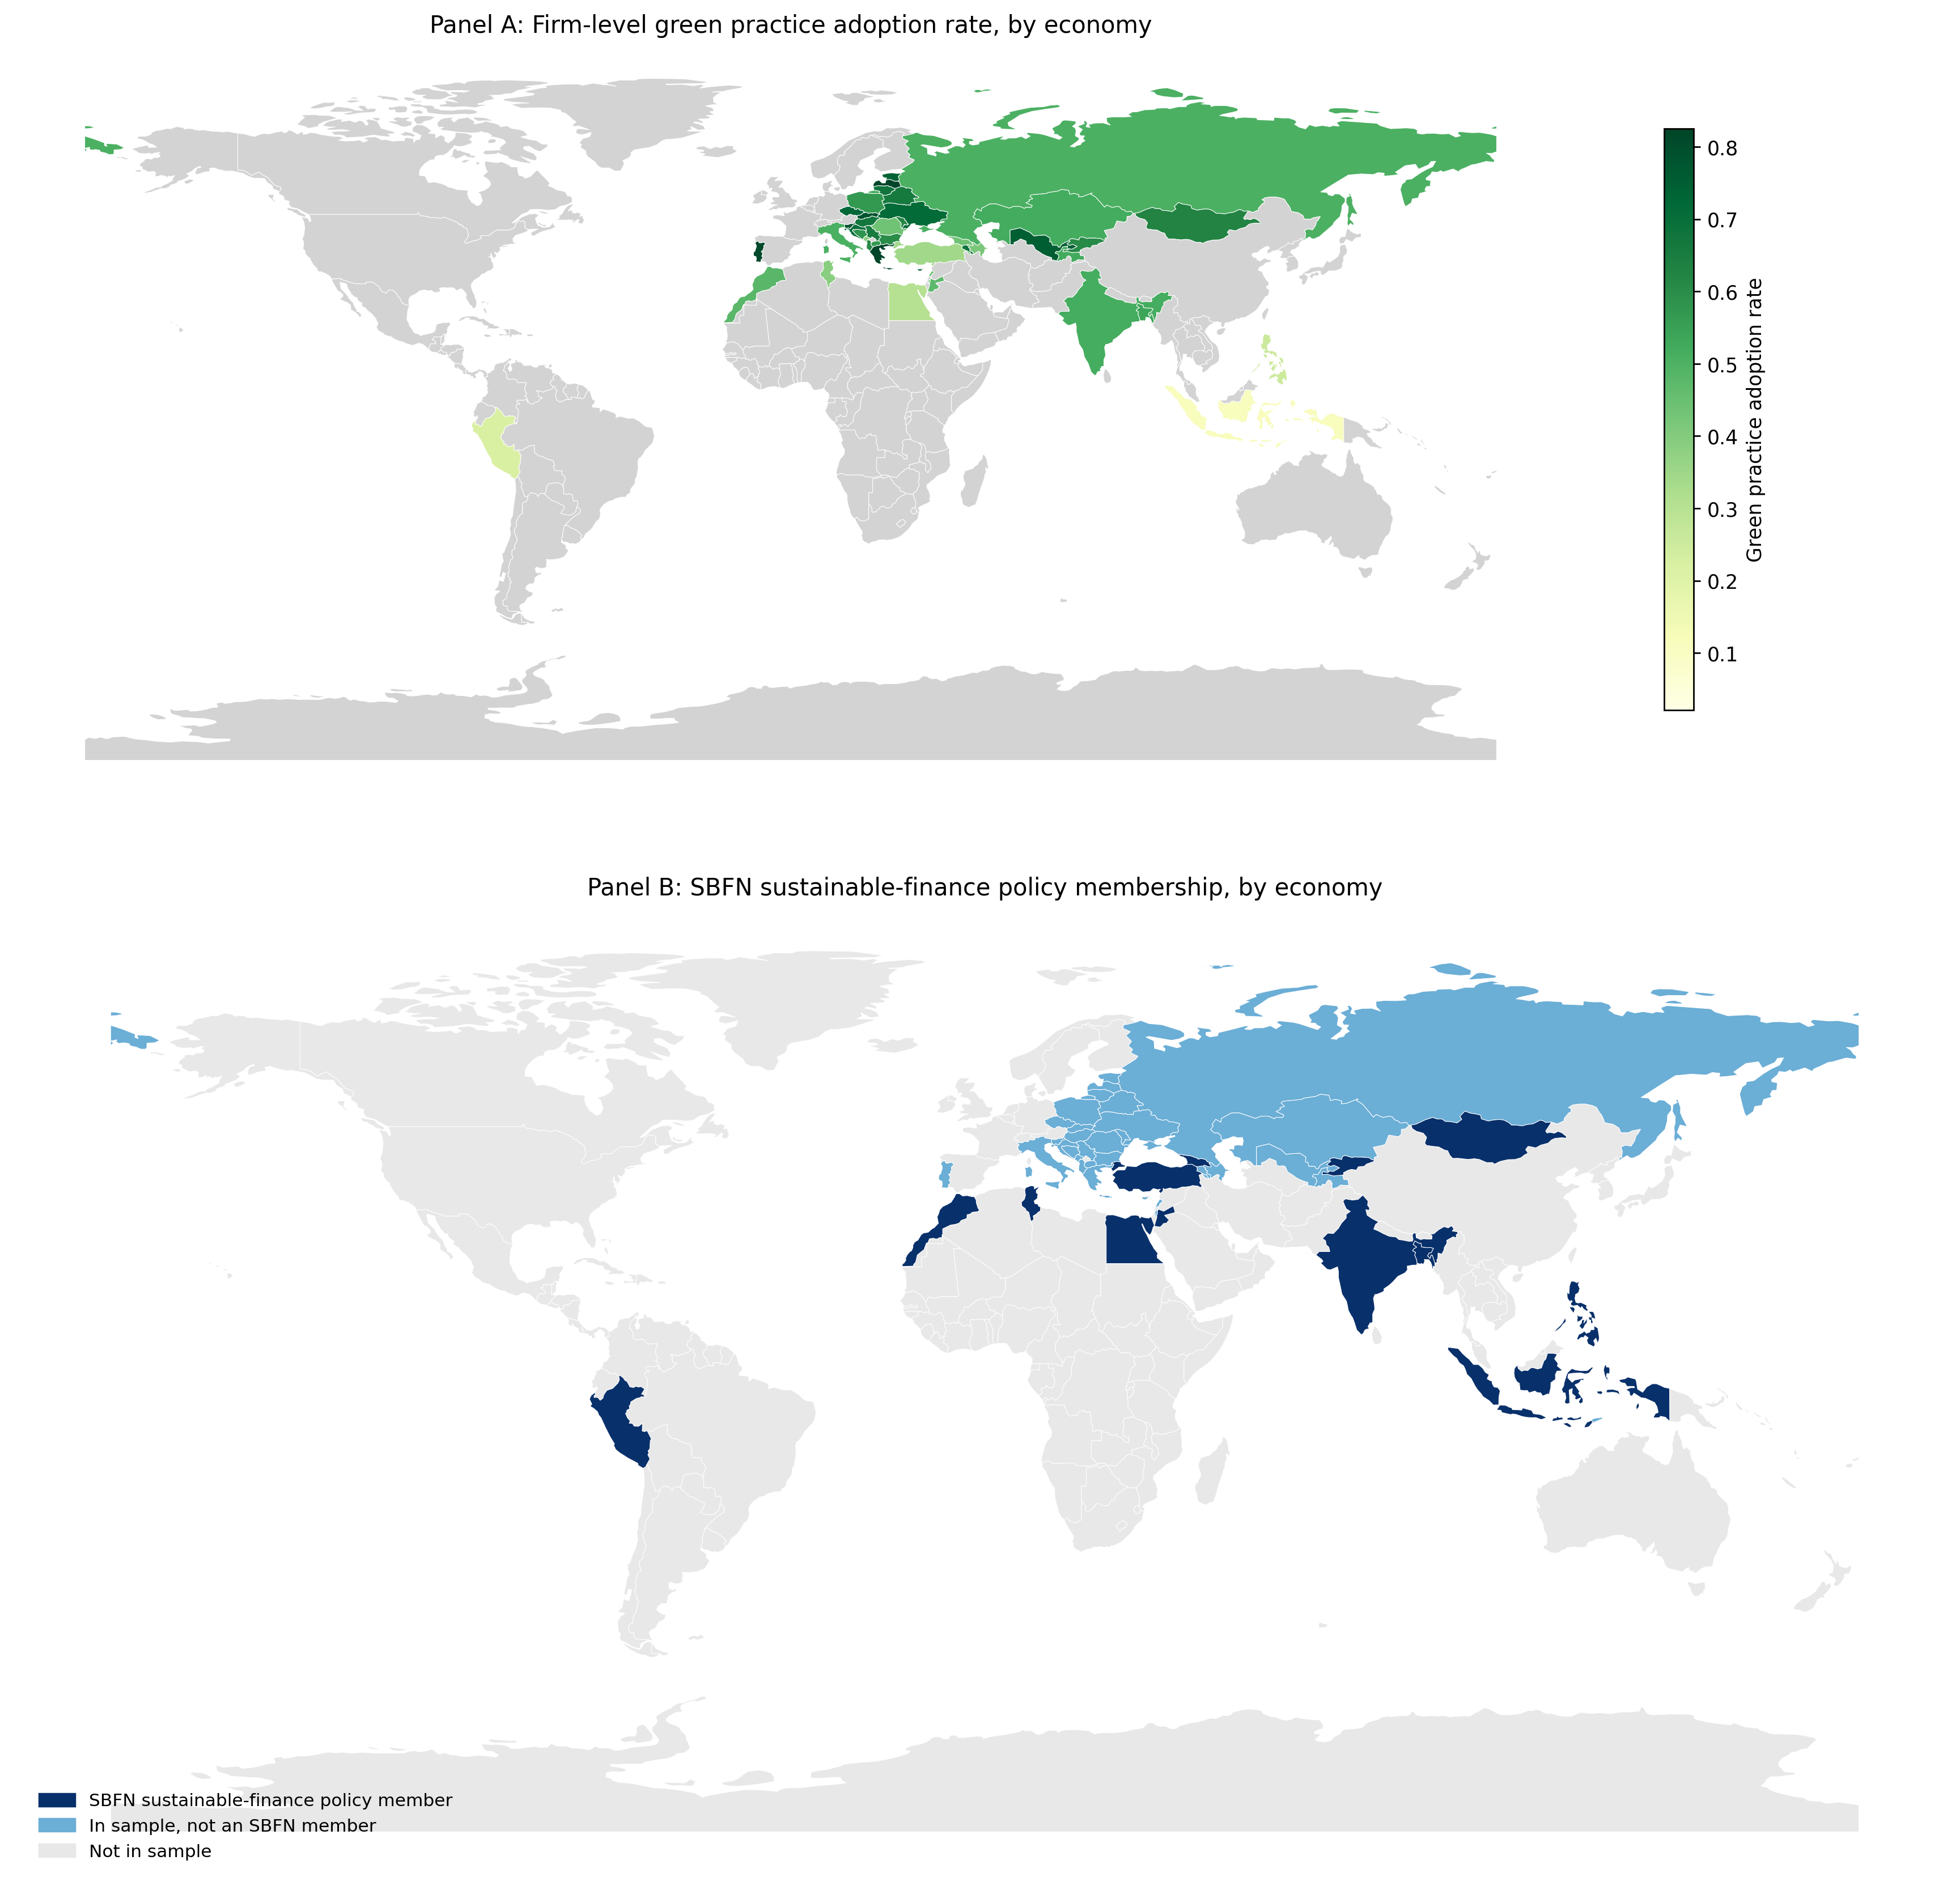
\includegraphics[width=0.85\textwidth,height=0.82\textheight,keepaspectratio]{../output/figures/fig1_world_map.png}
\caption{Green practice adoption and SBFN policy membership, by economy.}
\label{fig:map}
\end{figure}

\begin{figure}[htbp]
\centering
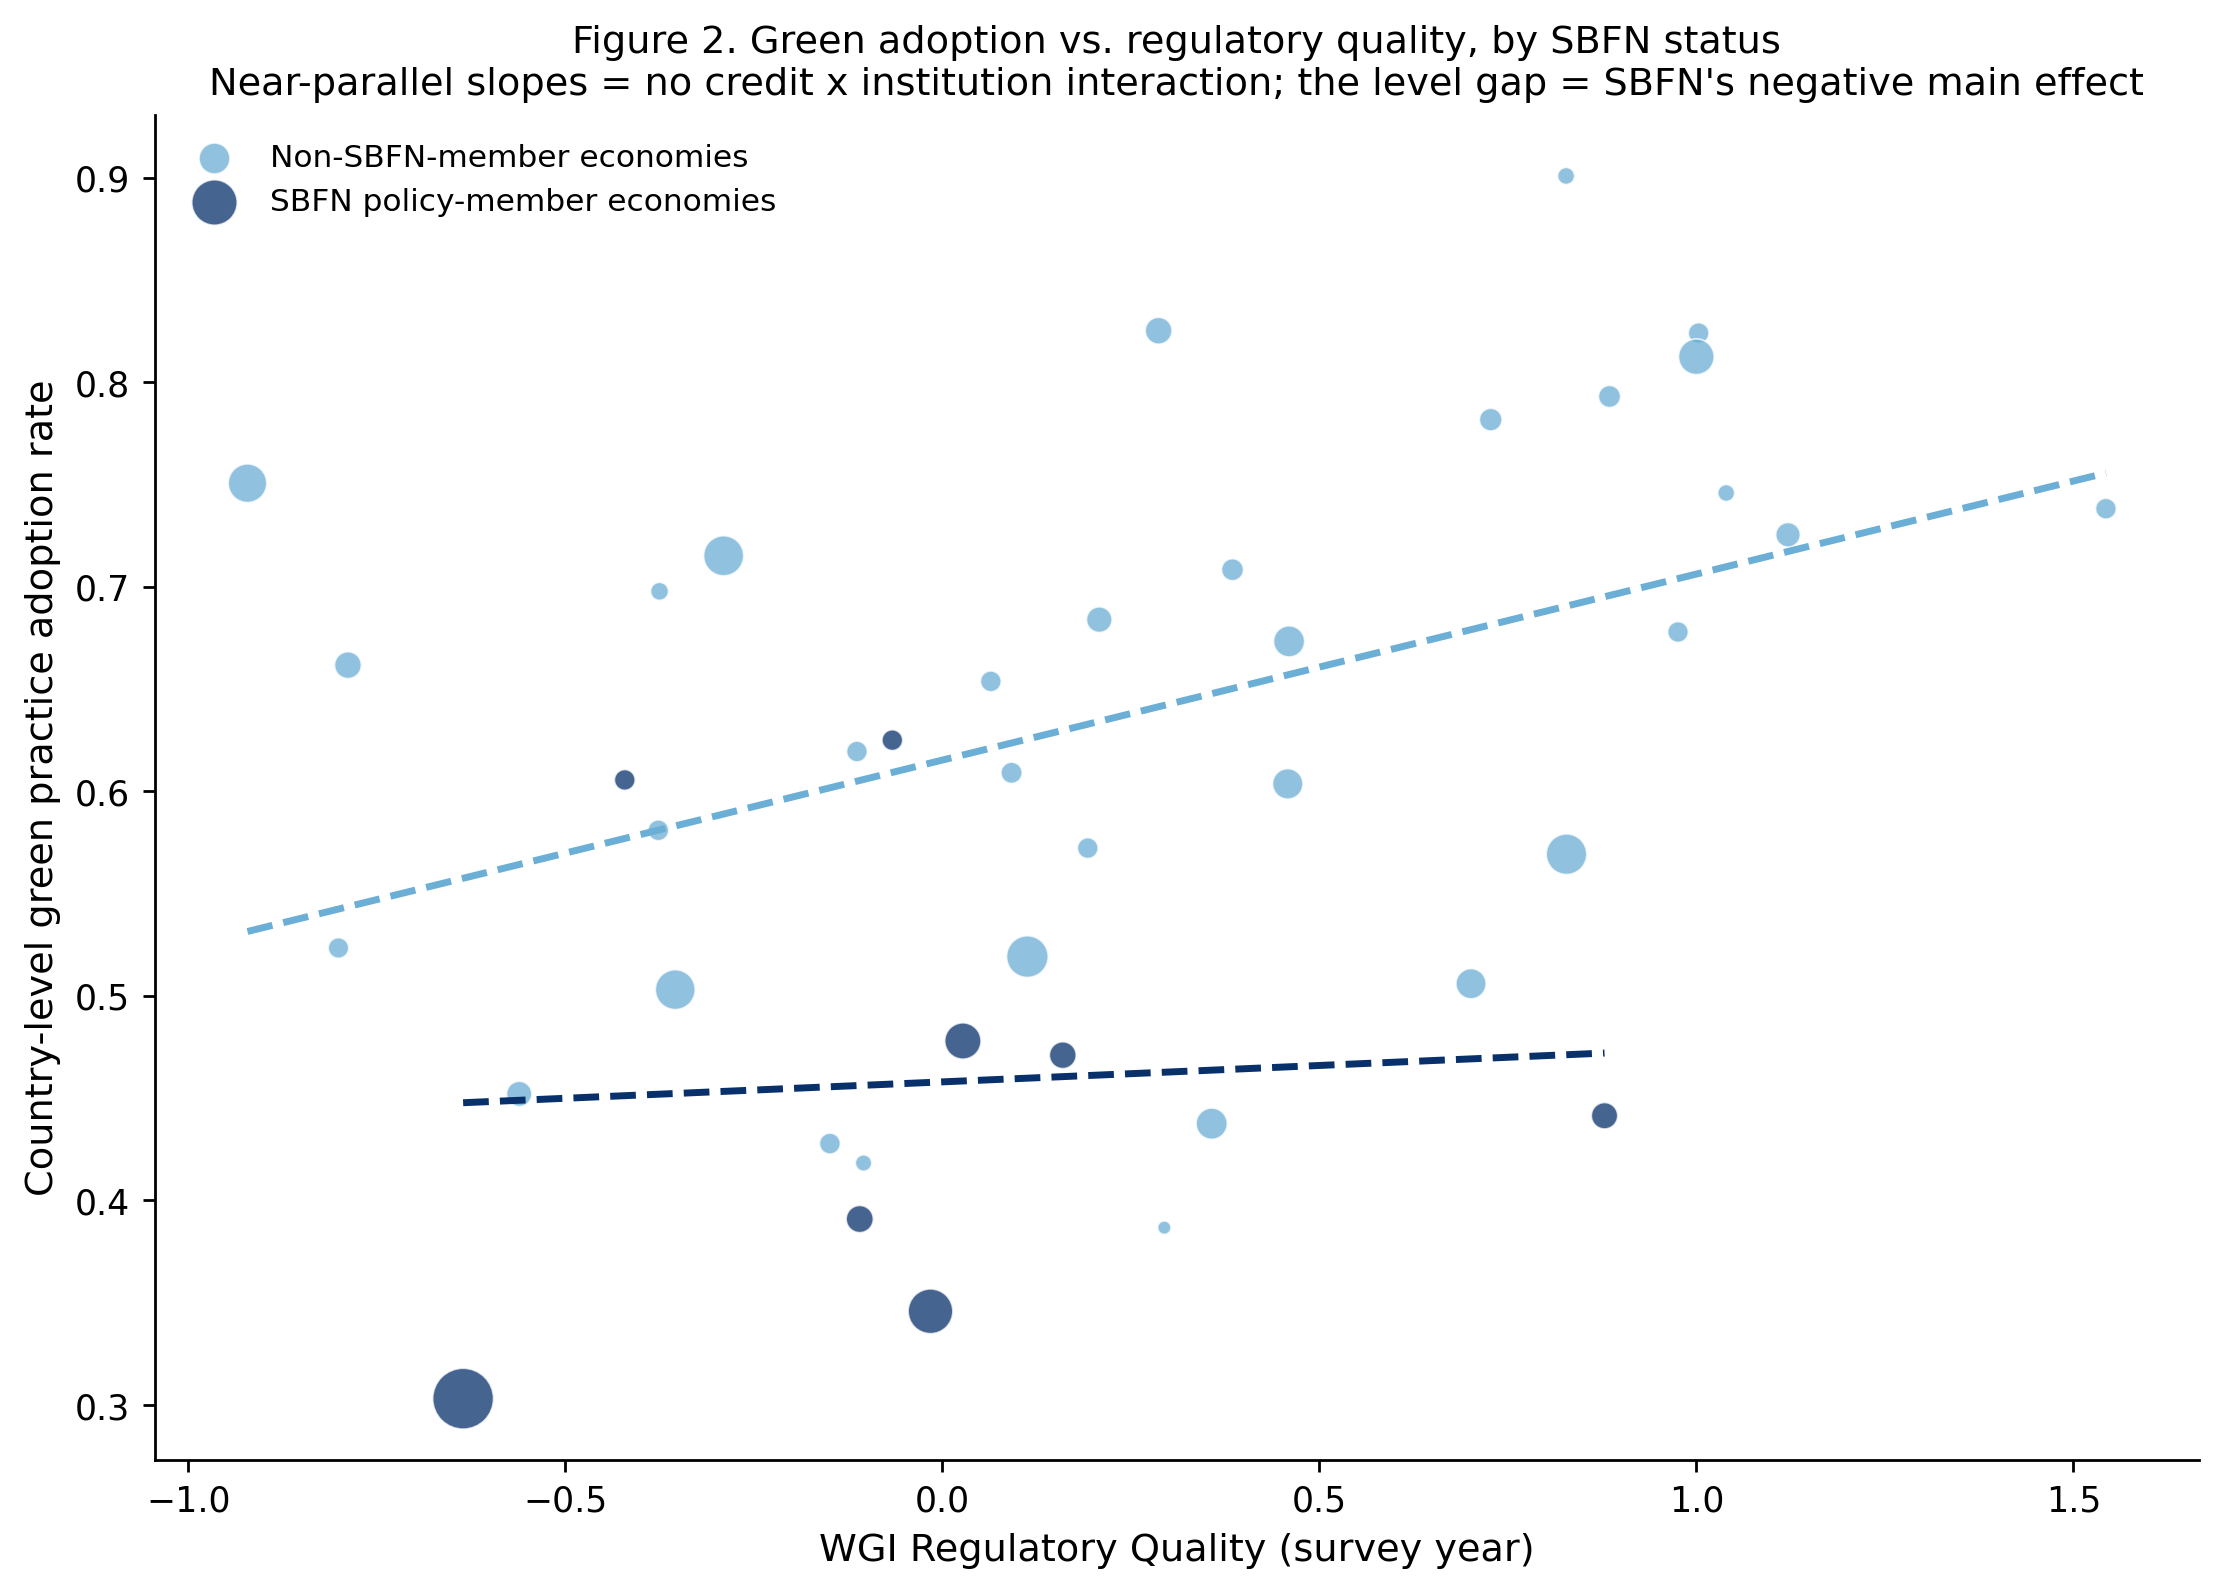
\includegraphics[width=0.85\textwidth]{../output/figures/fig2_scatter_regquality.png}
\caption{Green adoption vs. regulatory quality, by SBFN status.}
\label{fig:scatter}
\end{figure}

\subsection{Baseline classical benchmark}
\label{sec:baseline}

Table~\ref{tab:baseline} reports the pooled logistic baseline. Column M1 confirms H1 on its own terms: firms with a bank credit line are significantly more likely to have adopted a green practice ($b=0.571$, $p<0.001$; average marginal effect = 12.95 percentage points, 95\% CI [7.7, 18.2])---holding a formal credit line is associated with roughly the same increase in the probability of green adoption as moving from a small to a large firm, and a somewhat larger increase than being an exporter. Column M2 adds SBFN status and its interaction with credit access: the SBFN main effect is large, negative, and precisely estimated ($b=-0.991$, $p<0.001$), while the credit $\times$ SBFN interaction is small and statistically indistinguishable from zero ($b=0.049$, $p=0.773$). Column M3 adds the fully saturated triple interaction with regulatory quality, and it is this column, not the hierarchical model of Section~\ref{sec:multilevel}, that carries the paper's direct test of H3: the credit $\times$ SBFN $\times$ regulatory-quality term is small, wrong-signed relative to H3's prediction, and nowhere near significance ($b=-0.104$, $\text{se}=0.272$, $p=0.702$). The rest of M3 tells the same story at greater length: every interaction term involving credit access is small and insignificant, while regulatory quality's uninteracted relationship with adoption is positive, if only marginally significant in this particular fully-saturated specification ($b=0.278$, $p=0.110$).

As set out in Section~\ref{sec:methodology}, adding country fixed effects here would absorb the SBFN and regulatory-quality main effects entirely, while leaving the interaction terms identified but reliant on the contrast between within-country credit variation in this sample's eight adopter economies and its thirty-three non-adopters. Table~\ref{tab:baseline} accordingly reports main effects and interactions jointly, without country fixed effects; what it shows is a genuine test of H2 and, in M3, of H3, not a placeholder---and that test returns no interaction on either. The question the remaining two stages are built to answer is whether that null result reflects a real absence of policy moderation, or an artifact of forcing a two-level question through a single-level model with country-clustered standard errors computed over only 41 clusters, a setting in which such standard errors are known to be unreliable \citep{cameron2015}.

\begin{table}[htbp]
\centering
\caption{Baseline classical logit regressions (dependent variable: green practice adoption, binary). Country-clustered standard errors in parentheses.}
\label{tab:baseline}
\begin{footnotesize}
\begin{tabular}{lccc}
\toprule
 & M1 & M2 & M3 \\
\midrule
Credit access & 0.571*** & 0.459*** & 0.373*** \\
 & (0.123) & (0.090) & (0.085) \\
SBFN member & & -0.991*** & -0.844*** \\
 & & (0.178) & (0.209) \\
Credit $\times$ SBFN & & 0.049 & 0.019 \\
 & & (0.168) & (0.140) \\
Regulatory quality & & & 0.278 \\
 & & & (0.174) \\
Credit $\times$ Reg.\ quality & & & 0.144 \\
 & & & (0.142) \\
SBFN $\times$ Reg.\ quality & & & 0.053 \\
 & & & (0.261) \\
Credit $\times$ SBFN $\times$ Reg.\ quality & & & -0.104 \\
 & & & (0.272) \\
Log sales & 0.061 & 0.041 & 0.068** \\
 & (0.039) & (0.034) & (0.032) \\
Foreign owned & 0.219 & 0.244* & 0.220 \\
 & (0.143) & (0.139) & (0.143) \\
Exporter & 0.537*** & 0.471*** & 0.412*** \\
 & (0.092) & (0.074) & (0.079) \\
Sector, size controls & Yes & Yes & Yes \\
\midrule
$N$ & 23{,}914 & 23{,}914 & 23{,}914 \\
Pseudo $R^2$ & 0.058 & 0.089 & 0.093 \\
\bottomrule
\multicolumn{4}{l}{*** $p<0.01$, ** $p<0.05$, * $p<0.10$}
\end{tabular}
\end{footnotesize}
\end{table}

\subsection{Bayesian hierarchical model --- primary test of H2}
\label{sec:multilevel}

The hierarchical specification---country-varying random slopes on credit access, cross-level interactions with SBFN status and standardized regulatory quality, four chains of 1{,}000 post-warmup draws each, all $\hat{R}\leq1.01$ and $\text{ess}_{\text{bulk}}$ between 797 and 2{,}270---is built specifically to give H2 a fair hearing under inference the 41-cluster classical specification cannot deliver, and to test regulatory quality's own two-way moderation alongside it. H3's three-way claim is not tested here (Section~\ref{sec:methodology}); it is tested in Table~\ref{tab:baseline}'s M3 above and in Section~\ref{sec:global} below, and returns a null in both. This specification does not change the conclusion either. Table~\ref{tab:multilevel} reports the full posterior summary; three results stand out.

First, the firm-level credit effect (H1) survives unchanged in substance: posterior mean 0.33 (89\% equal-tailed interval [0.18, 0.49]), comfortably excluding zero. Second, both country-level institutional variables retain clean, precisely estimated \emph{main} effects on the baseline adoption rate---SBFN membership net-negative (-0.57, 89\% ETI [-1.00, -0.09]), regulatory quality net-positive (0.34, 89\% ETI [0.16, 0.53])---reproducing, with proper hierarchical uncertainty quantification rather than an absorbed or clustered approximation, exactly the level-shift pattern Figure~\ref{fig:scatter} shows visually. Third, and centrally for H2, neither cross-level interaction is distinguishable from zero: credit $\times$ SBFN, 0.072 (89\% ETI [-0.26, 0.40]); credit $\times$ regulatory quality (standardized), 0.004 (89\% ETI [-0.13, 0.14])---a near-exact zero on the latter, not merely an imprecise one. The first of these is the direct H2 test; the second establishes that regulatory quality does not moderate the credit-green channel on its own, which is a necessary condition for the mechanism H3 posits without being a test of H3 itself.

We read this as an honest and, we think, informative finding rather than a disappointing one: giving the moderation hypothesis a hierarchical model built for precisely this two-level question still returns no interaction, while sharpening (relative to the pooled baseline) the confidence with which we can state that SBFN status and regulatory quality shift the \emph{level} of green adoption directly.

\begin{table}[htbp]
\centering
\caption{Bayesian hierarchical model, posterior summary (four chains, 1{,}000 post-warmup draws each).}
\label{tab:multilevel}
\begin{tabular}{lccccc}
\toprule
Parameter & Mean & SD & 89\% ETI low & 89\% ETI high & $\hat{R}$ \\
\midrule
Intercept & -1.93 & 0.246 & -2.30 & -1.50 & 1.00 \\
Credit access & 0.33 & 0.097 & 0.18 & 0.49 & 1.00 \\
SBFN member & -0.57 & 0.300 & -1.00 & -0.09 & 1.01 \\
Credit $\times$ SBFN & 0.072 & 0.211 & -0.26 & 0.40 & 1.00 \\
Reg.\ quality (std.) & 0.344 & 0.116 & 0.16 & 0.53 & 1.00 \\
Credit $\times$ Reg.\ quality & 0.004 & 0.087 & -0.13 & 0.14 & 1.00 \\
\bottomrule
\end{tabular}
\end{table}

\subsection{Causal forest / heterogeneous treatment effects}
\label{sec:causalforest}

Table~\ref{tab:causalforest} and Figure~\ref{fig:cateplot} report the Causal Forest DML estimates, which impose no linear-interaction functional form and let the treatment effect vary flexibly across firm and country covariates. The overall average treatment effect of credit access is 0.073 (95\% CI [-0.040, 0.186])---directionally consistent with, though smaller in magnitude and less precisely estimated than, the logit average marginal effect of 0.130 in Section~\ref{sec:baseline}, reflecting the more conservative variance properties of a doubly-robust, cross-fitted nonparametric estimator relative to a parametric logit on the same data. Critically, the conditional average treatment effects triangulate with Section~\ref{sec:multilevel} rather than contradicting it: the estimated effect is 0.072 for firms in non-SBFN economies versus 0.076 for firms in SBFN economies, and 0.075 / 0.070 / 0.075 across the low/middle/high regulatory-quality terciles respectively---three different institutional cuts, three essentially flat effects, all visibly overlapping in Figure~\ref{fig:cateplot}. Two entirely independent estimators, one parametric and hierarchical, one nonparametric and forest-based, agree on the absence of institutional moderation.

The forest's feature-importance decomposition adds a genuinely new result rather than only confirming the null, and speaks directly to the auxiliary H4 introduced in Section~\ref{sec:h4}: of the four candidate effect-modifiers, firm size (log sales) accounts for 75.6\% of the model's explained heterogeneity, versus 19.9\% for regulatory quality, 2.6\% for SBFN status, and 1.9\% for exporter status. Whatever heterogeneity exists in how strongly credit access predicts green adoption is, on this evidence, primarily a firm-level rather than a country-institutional phenomenon, supporting H4. Collapsing this into the Enterprise Surveys' own coarse size strata, however, does not reveal a clean monotonic gradient: the estimated effect is 0.080 for small firms, 0.075 for medium firms, and 0.057 for large firms (Table~\ref{tab:sizecate}; all with wide, overlapping confidence intervals spanning zero), which if anything runs opposite to a simple ``larger firms better absorb a green investment's fixed costs'' story rather than confirming it. Read alongside the 75.6\% importance share for the continuous size measure, we take this as evidence that the heterogeneity the forest is detecting is more granular or non-monotonic across the firm-size distribution than a three-category collapse can reveal, rather than evidence for any particular direction of a size gradient---a qualification we report explicitly rather than paper over with a tidier-sounding but unsupported claim. This redirects, rather than closes, the paper's institutional-moderation question, and we return to it in Section~\ref{sec:discussion}.

\begin{table}[htbp]
\centering
\caption{Causal forest DML: average treatment effect, CATEs, and feature importances.}
\label{tab:causalforest}
\begin{tabular}{lccc}
\toprule
Estimate & Value & 95\% CI low & 95\% CI high \\
\midrule
Overall ATE & 0.0733 & -0.0396 & 0.1862 \\
CATE $\vert$ SBFN non-member & 0.0723 & -0.0300 & 0.1746 \\
CATE $\vert$ SBFN member & 0.0758 & -0.0591 & 0.2107 \\
CATE $\vert$ reg.\ quality tercile: low & 0.0753 & -0.0568 & 0.2075 \\
CATE $\vert$ reg.\ quality tercile: mid & 0.0697 & -0.0355 & 0.1749 \\
CATE $\vert$ reg.\ quality tercile: high & 0.0749 & -0.0203 & 0.1701 \\
\midrule
Feature & Importance & & \\
\midrule
SBFN member & 0.0257 & & \\
Regulatory quality & 0.1993 & & \\
Log sales & 0.7562 & & \\
Exporter dummy & 0.0189 & & \\
\bottomrule
\end{tabular}
\end{table}

\begin{table}[htbp]
\centering
\caption{Causal forest CATEs by firm-size category.}
\label{tab:sizecate}
\begin{tabular}{lccc}
\toprule
Size category & CATE & 95\% CI low & 95\% CI high \\
\midrule
Small & 0.0797 & -0.0409 & 0.2004 \\
Medium & 0.0747 & -0.0344 & 0.1838 \\
Large & 0.0569 & -0.0428 & 0.1565 \\
\bottomrule
\end{tabular}
\end{table}

\subsection{Small-sample supplementary check: waste-minimization adoption}
\label{sec:extension}

Before turning to the global-sample replication that is this paper's second major test (Section~\ref{sec:global}), we report a smaller supplementary check using waste-minimization adoption---an outcome not captured in the standardized cross-country database underlying the global sample, and so a genuinely independent (if small-sample) data point---available in four economies whose Green Economy modules asked this item under directly comparable wording: India 2022, Indonesia 2023, Peru 2023, and Timor-Leste 2021 (descriptive rates in Supplementary Table~S1). Three of these four are themselves SBFN members, so this sample cannot re-test the SBFN-adoption contrast; what it can test is whether the credit-to-green channel documented in Sections~\ref{sec:baseline}--\ref{sec:causalforest} generalizes beyond the ECA-MENA sample. It does: pooled across the four economies, having an overdraft facility is associated with significantly higher odds of waste-minimization adoption ($b=0.422$, $p<0.001$, $N=9{,}038$, 4 countries)---a preview, on a different continent and half-decade, of the much larger replication in Section~\ref{sec:global}.

\subsection{Additional robustness}
\label{sec:robustness}

Supplementary Table~S2 subjects the primary-sample finding to four further checks (sector fixed effects, firm controls, country-clustered standard errors; no country fixed effects, for the reason given in Section~\ref{sec:methodology}). Replacing the binary outcome with the continuous seven-item green-adoption index reproduces the same pattern by OLS. Replacing bank credit access with two alternative finance measures produces one point of nuance: using overdraft-facility access, the overdraft $\times$ SBFN interaction is negative and significant ($b=-0.346$, $p=0.031$)---the one interaction term in the paper that clears a conventional significance threshold, and it runs opposite to H2's predicted direction---whereas using the reverse-coded perceived finance-obstacle measure, both the main effect and its SBFN interaction are precisely zero. Splitting the sample into manufacturing and services subsamples shows the credit-access main effect and the null credit $\times$ SBFN interaction replicate within each sector separately. We read the overdraft result as suggestive rather than conclusive: it is one significant coefficient among more than a dozen interaction tests across the paper, and a Benjamini--Hochberg false-discovery-rate correction applied to that full family (Supplementary Table~S3) pushes its raw $p=0.031$ to $p=0.403$---no coefficient in the family survives at a false discovery rate of 0.10 or even 0.40, exactly what a pure false-discovery process would be expected to produce roughly one time in twenty.

\subsection{Global-sample replication with country fixed effects}
\label{sec:global}

The preceding five subsections establish the paper's central finding on the primary sample. We now subject that finding to what we consider the most demanding test available to us: complete re-estimation on an independently assembled, 162-economy global sample (Section~\ref{sec:methodology}), using a different outcome variable (CO2-emissions monitoring rather than the seven-item composite), different survey years (2021--2026 rather than 2018--2020), and, for the first time in the paper, a country-fixed-effects specification that this much larger set of clusters can support. Figure~\ref{fig:globalmap} maps the combined reach of the two samples together: 166 distinct economies, spanning every region and, through the global sample specifically, extending for the first time in this literature into high-income economies with no SBFN involvement at all.

Table~\ref{tab:global} reports two specifications. Column M1, without country fixed effects, is the direct global-sample analogue of Table~\ref{tab:baseline}'s primary-sample baseline: credit access remains positive and significant ($b=0.198$, $p=0.039$, $N=89{,}797$, 159 countries), while the SBFN main effect ($b=-0.171$, $p=0.353$), the credit $\times$ SBFN interaction ($b=0.278$, $p=0.430$), and every regulatory-quality interaction are statistically indistinguishable from zero. Like Table~\ref{tab:baseline}'s M3, this specification is fully saturated and so retains the credit $\times$ SBFN $\times$ regulatory-quality term H3 requires, which is likewise insignificant; Table~\ref{tab:global} tabulates the focal two-way terms only. H3 therefore receives a direct, fully saturated test on both firm-level samples, and returns a null on each. Column M2 imposes country fixed effects, absorbing the SBFN and regulatory-quality main effects by construction (they are collinear with $\delta_c$, since both are constant within a given country-year) while leaving their firm-level interactions with credit access fully identified, because credit access itself varies within country. This is a sharper test than anything the primary sample's single 2018--2020 wave can support, and it returns the same answer with even more precision: credit access is strongly significant ($b=0.249$, $p<0.001$), while the credit $\times$ SBFN interaction ($b=0.506$, $p=0.205$) and the credit $\times$ regulatory-quality interaction ($b=-0.044$, $p=0.346$) remain null.

We regard this as the paper's most important robustness result. It is not a re-analysis of the same data under a different label: it is a different outcome construct, a different set of economies (only a handful of which overlap with the primary sample), a different half-decade, and an econometric specification --- country fixed effects --- that is only available at all because this second sample has enough clusters to support it. That the qualitative conclusion is identical across both samples and across the full set of four estimators reported in this paper (classical logit, Bayesian hierarchical, causal forest, and now country-fixed-effects logit) is, we think, considerably stronger evidence for the paper's central claim than either sample could offer alone.

\begin{figure}[htbp]
\centering
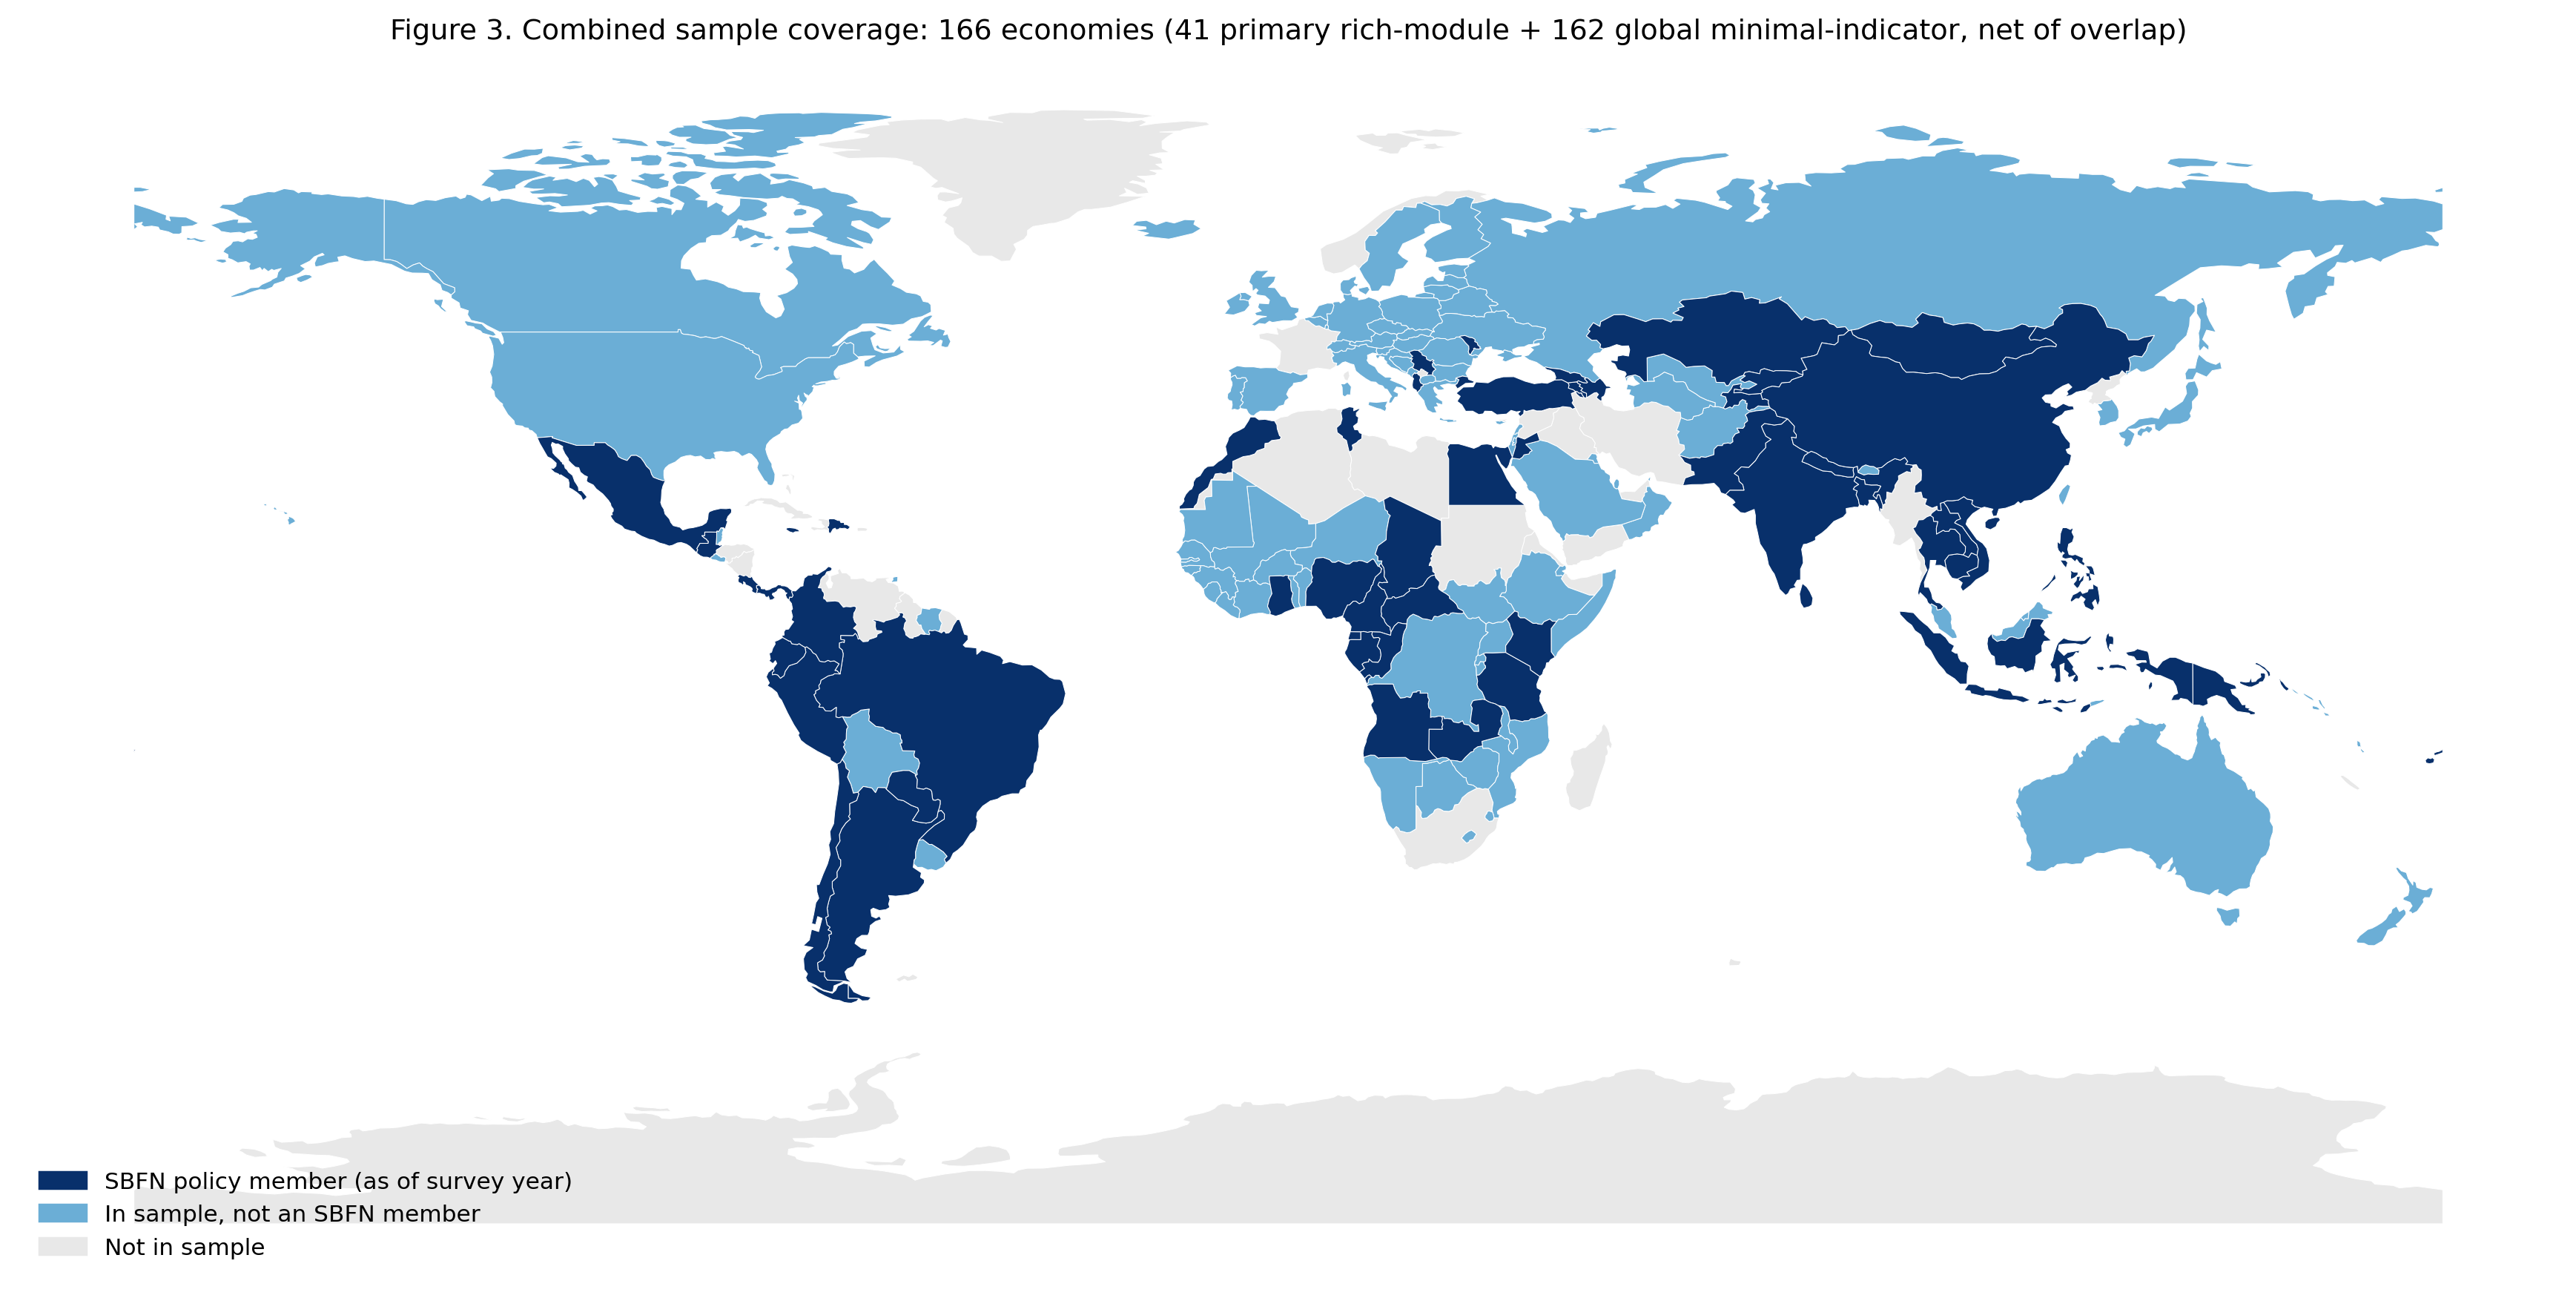
\includegraphics[width=0.95\textwidth]{../output/figures/fig3_global_map.png}
\caption{Combined sample coverage: 166 economies (41 primary + 162 global, net of overlap), shaded by SBFN status.}
\label{fig:globalmap}
\end{figure}

\begin{table}[htbp]
\centering
\caption{Global-sample regressions (dependent variable: CO2-emissions monitoring, binary). Country-clustered standard errors in parentheses; M2's SBFN and regulatory-quality main effects are absorbed by country fixed effects and are not separately estimable.}
\label{tab:global}
\begin{tabular}{lcc}
\toprule
 & M1: no country FE & M2: country FE \\
\midrule
Credit access & 0.198** & 0.249*** \\
 & (0.096) & (0.057) \\
SBFN member & -0.171 & --- (absorbed) \\
 & (0.184) & \\
Credit $\times$ SBFN & 0.278 & 0.506 \\
 & (0.352) & (0.399) \\
Regulatory quality (std.) & 0.155 & --- (absorbed) \\
 & (0.096) & \\
Credit $\times$ Reg.\ quality & 0.092 & -0.044 \\
 & (0.089) & (0.047) \\
Log sales & 0.127*** & 0.288*** \\
 & (0.027) & (0.028) \\
Foreign owned & 0.621*** & 0.528*** \\
 & (0.083) & (0.046) \\
Exporter & 0.456*** & 0.335*** \\
 & (0.094) & (0.044) \\
Country fixed effects & No & Yes \\
\midrule
$N$ & 89{,}797 & 89{,}797 \\
Countries & 159 & 159 \\
\bottomrule
\multicolumn{3}{l}{\footnotesize *** $p<0.01$, ** $p<0.05$, * $p<0.10$. Taiwan dropped (no WGI coverage).}
\end{tabular}
\end{table}

\subsection{Results summary across all specifications}
\label{sec:summary}

Sections~\ref{sec:baseline}--\ref{sec:global} report ten tables spanning four estimators and two independent samples. Figure~\ref{fig:coefplot} consolidates every coefficient bearing on H1--H3 into a single view. Panel A shows the credit-access effect (H1): every point estimate is positive and every confidence interval excludes zero, in both samples and all four estimators. Panels B and C show the credit $\times$ SBFN and credit $\times$ regulatory-quality interactions (H2, H3): every single confidence interval, across both samples and every estimator, straddles zero. Figure~\ref{fig:cateplot} shows the same non-result from a completely different angle---the causal forest's conditional average treatment effects broken out by SBFN status, regulatory-quality tercile, and firm-size category all overlap both each other and the overall average treatment effect. No subgroup split, by any variable examined in this paper, recovers a distinguishable effect.

\begin{figure}[htbp]
\centering
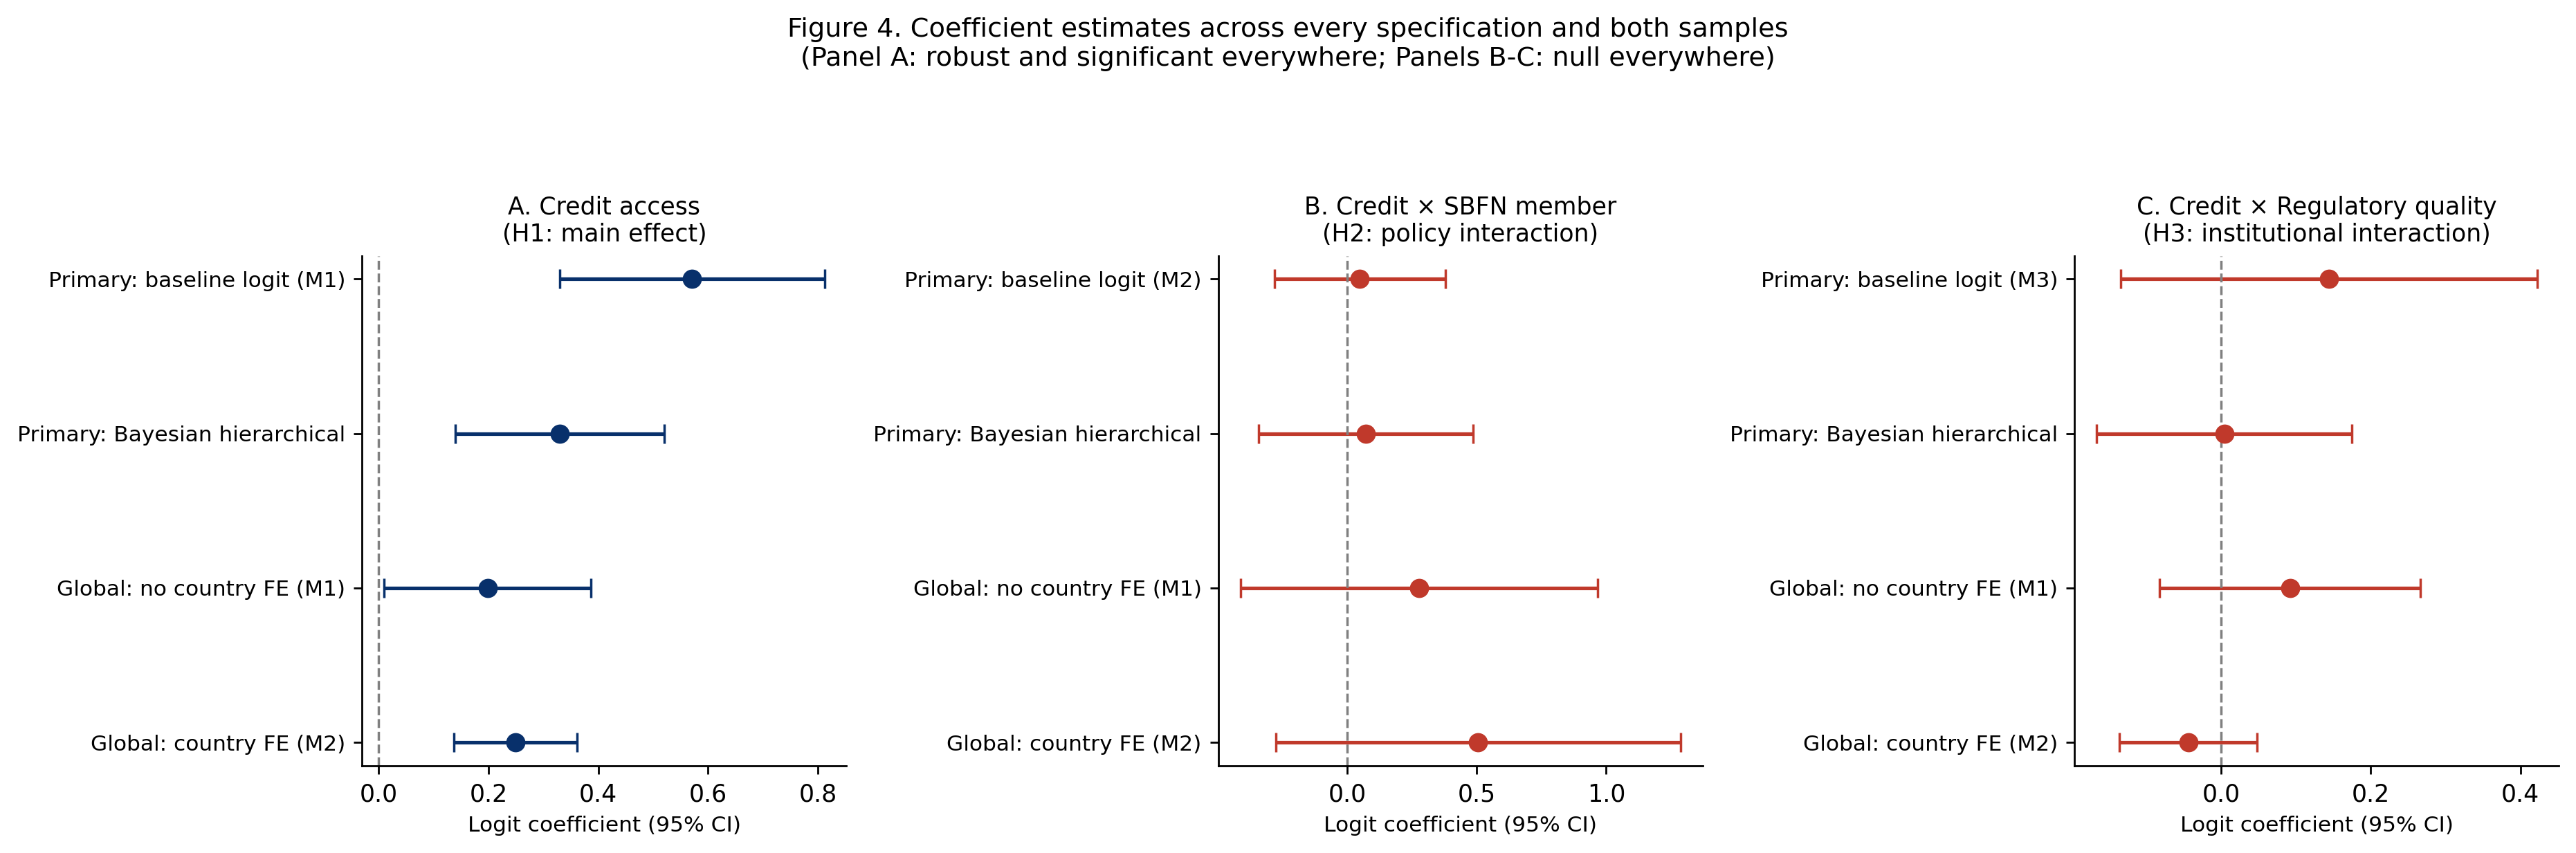
\includegraphics[width=0.98\textwidth]{../output/figures/fig4_coefficient_plot.png}
\caption{Coefficient estimates across every specification and both samples.}
\label{fig:coefplot}
\end{figure}

\begin{figure}[htbp]
\centering
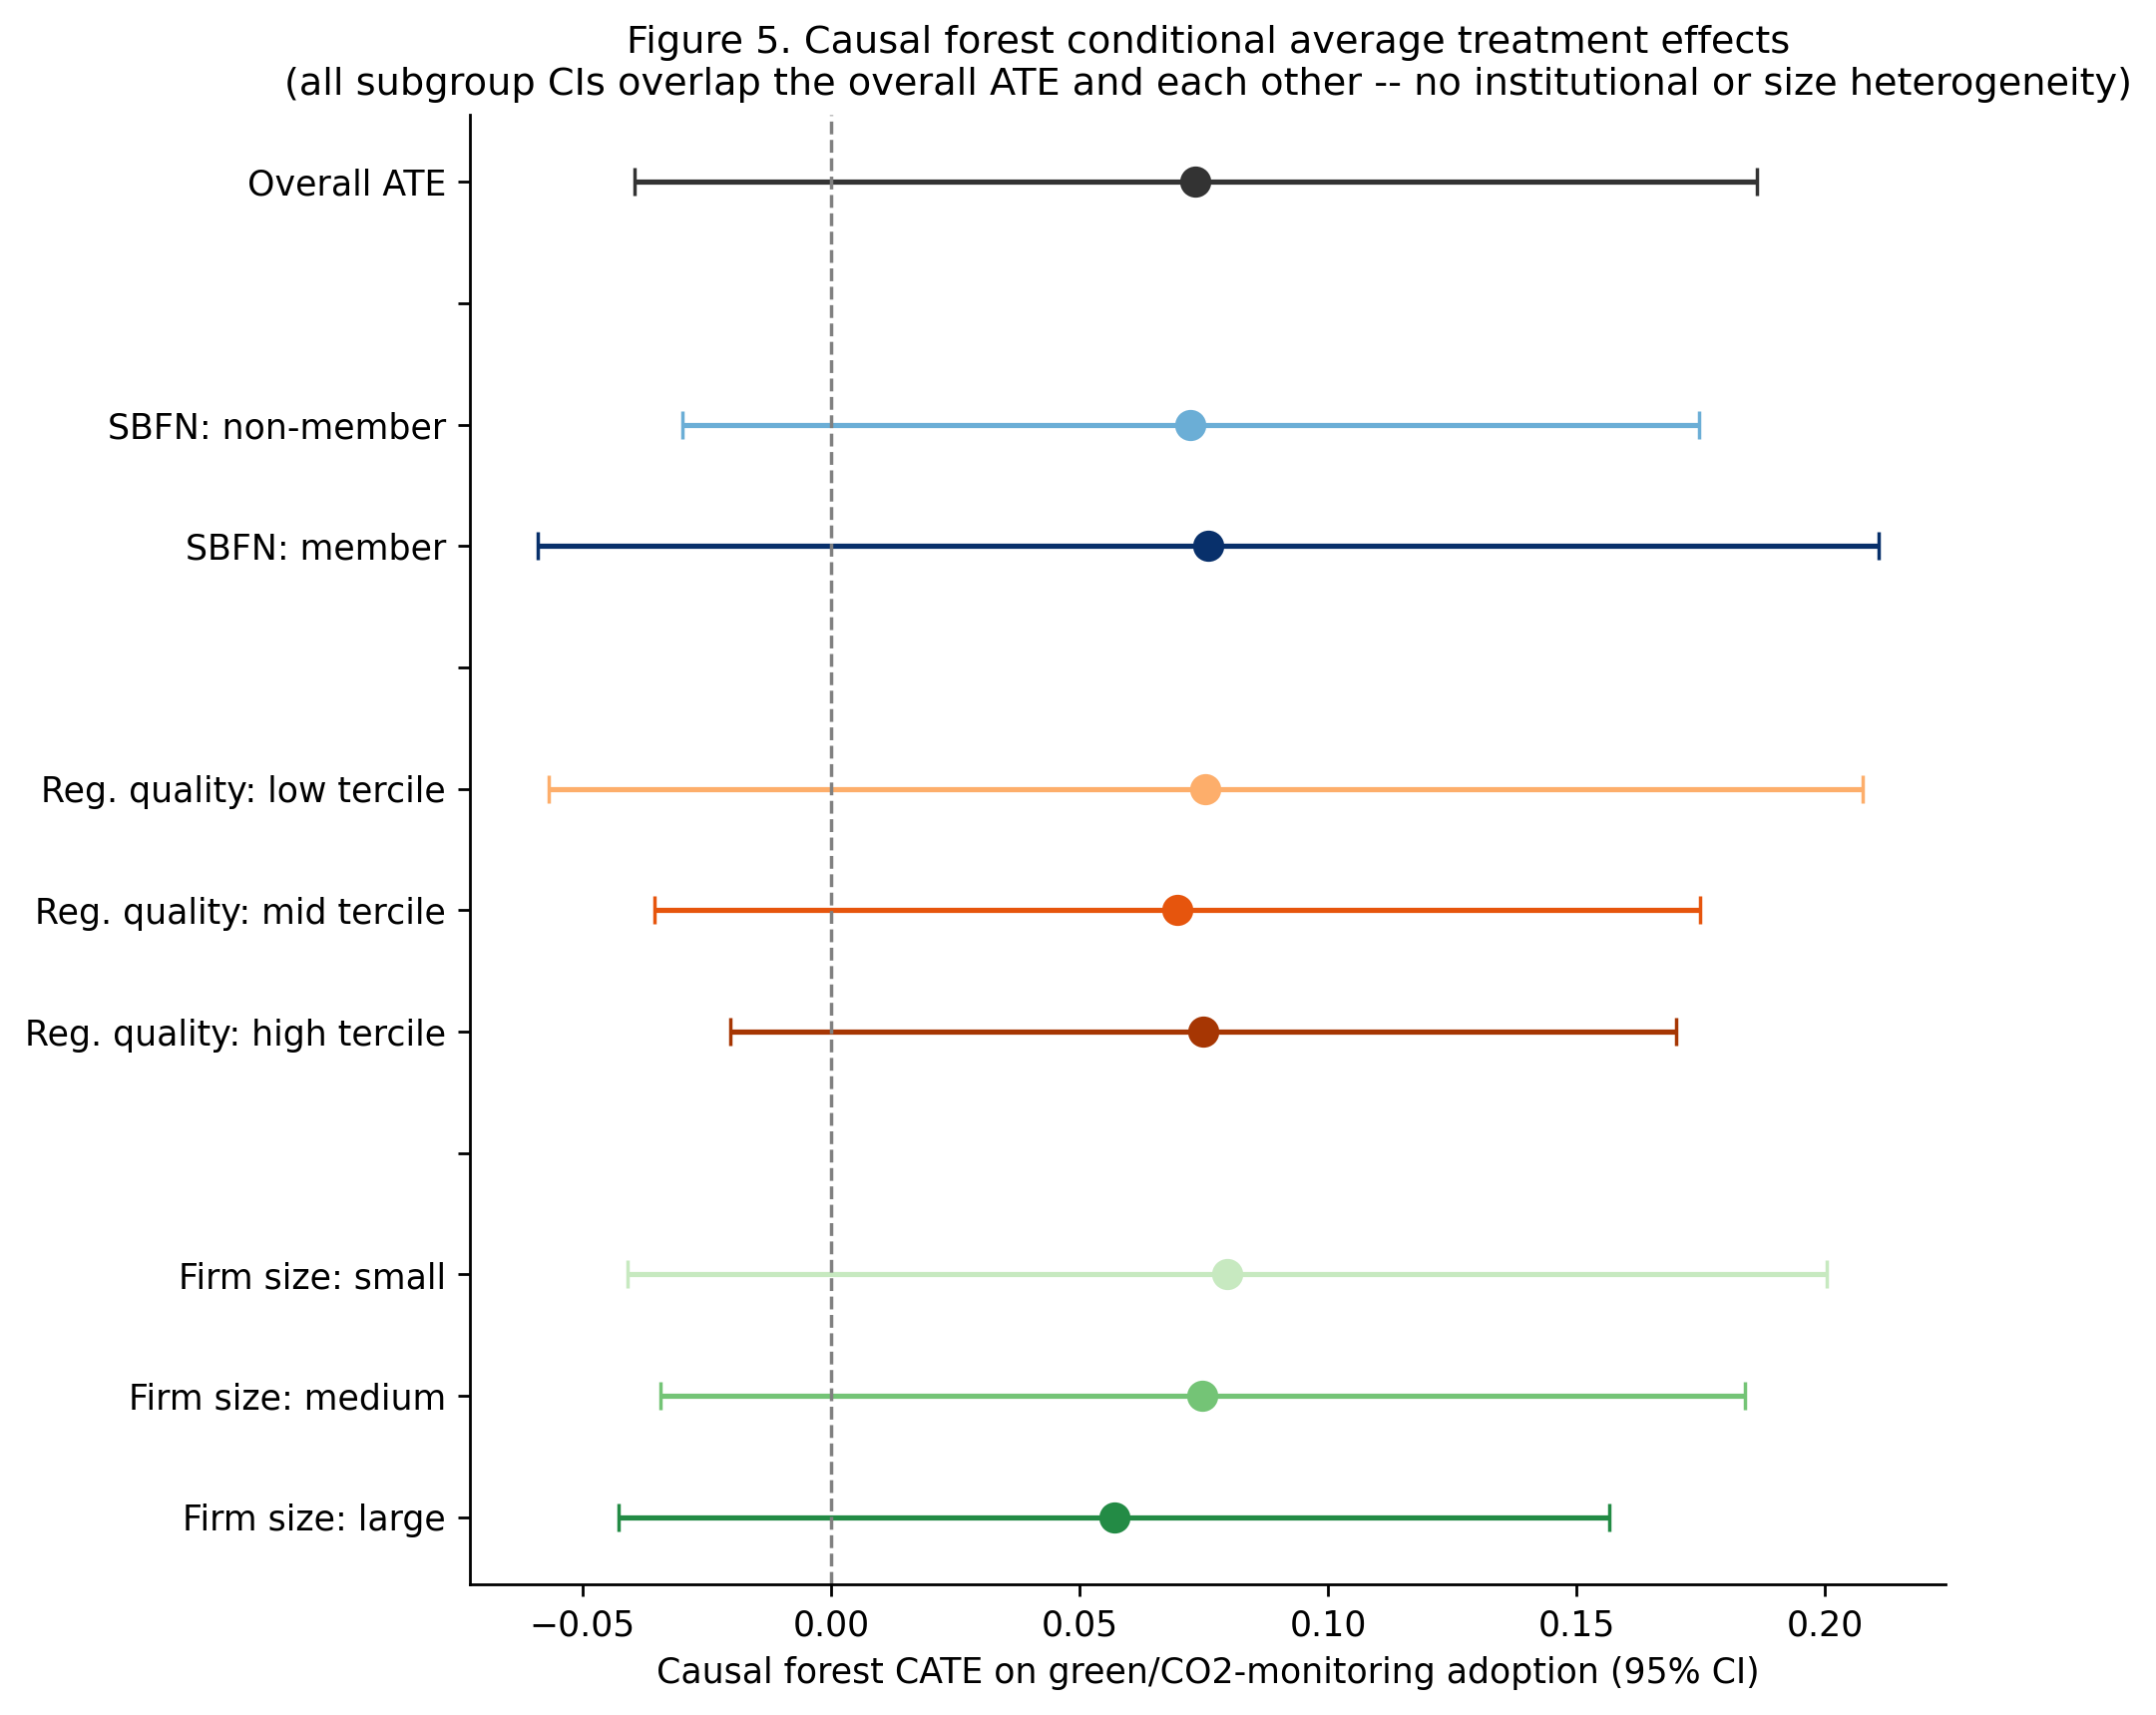
\includegraphics[width=0.75\textwidth]{../output/figures/fig5_cate_plot.png}
\caption{Causal forest conditional average treatment effects, by subgroup.}
\label{fig:cateplot}
\end{figure}

\section{Supplementary evidence: a country-level staggered event-study on macro environmental outcomes}
\label{sec:macrodid}

Sections~\ref{sec:baseline}--\ref{sec:summary} establish this paper's central finding using firm-level cross-sectional data, for the data-availability reasons given in Section~\ref{sec:methodology}: the WBES Green Economy module cannot support a staggered difference-in-differences or event-study design around each economy's own SBFN adoption date, because it has not been fielded as a repeated panel instrument. That constraint applies to the firm-level finance-to-green-investment channel specifically; it does not apply to a different, complementary question that the same SBFN adoption-timing variation can answer directly: does a country's aggregate environmental trajectory shift around its own SBFN adoption date? This section builds and reports that test, using an entirely independent data source and unit of analysis, precisely because it is the identification strategy this literature most often asks for, and because a genuine answer, however it comes out, is more useful than leaving the question unaddressed.

\subsection{Data and design}
\label{sec:macrodidmethod}

We assemble a country-year panel spanning every World Bank member economy with a non-aggregate ISO3 code (217 economies), 2000--2024. Treatment timing is each economy's SBFN join year, drawn from the same SBFN data portal membership roster used to construct the global sample (Section~\ref{sec:methodology}) and cross-checked against the global-sample SBFN coding used in Section~\ref{sec:global} (zero disagreements across 61 overlapping economies); economies that have never joined SBFN, as of the roster's most recent update, serve as the never-treated comparison group. This yields 68 ever-treated economies (join years 2012--2024, the same real staggered-adoption variation described in Section~\ref{sec:institutions}) and 149 never-treated economies. Outcome data come from the World Bank's World Development Indicators, retrieved via the World Bank DataBank API: renewable energy consumption (\% of total final energy consumption, \texttt{EG.FEC.RNEW.ZS}) and CO2 emissions per capita (AR5 GWP-consistent series, \texttt{EN.GHG.CO2.PC.CE.AR5}), both available for the large majority of economies from 2000 through at least 2021--2024. We additionally draw on GDP per capita (constant 2015 US\$, \texttt{NY.GDP.PCAP.KD}) as a covariate, to net out the obvious confound that SBFN-adopting economies are disproportionately still-industrializing, faster-growing economies whose emissions profiles are shaped by their development stage independently of any banking-sector policy.

We estimate the effect of SBFN adoption on each outcome using the Callaway and Sant'Anna (2021) staggered-adoption difference-in-differences estimator \citep{callaway2021}, which recovers group-time average treatment effects for each adoption cohort separately and aggregates them into an overall average treatment effect on the treated (ATT) and an event-study profile. We report this estimator, rather than a standard two-way-fixed-effects (TWFE) regression, because TWFE is now well known to produce badly biased estimates under staggered treatment timing when already-treated units are implicitly used as controls for later-treated units \citep{goodmanbacon2021}; we report a naive TWFE specification alongside the Callaway-Sant'Anna estimates specifically to illustrate the size of that bias in our own data, rather than as a candidate preferred estimate. For each outcome we report both an unconditional specification and a doubly-robust specification conditioning on log GDP per capita, and we check the doubly-robust specification's sensitivity to the choice of comparison group, using never-treated economies as our preferred comparison group throughout and not-yet-treated economies (those that will eventually adopt but had not yet, as of the relevant relative period) as a robustness check.

\subsection{Results}
\label{sec:macrodidresults}

Table~\ref{tab:macrodid} reports the overall ATT for both outcomes across four specifications, including a comparison-group robustness check; Figure~\ref{fig:macroevent} plots the full event-study profile (doubly-robust, GDP-per-capita-controlled, never-treated specification) for both outcomes.

\begin{table}[htbp]
\centering
\caption{Country-level staggered event-study: overall average treatment effect of SBFN adoption on macro environmental outcomes. Callaway-Sant'Anna estimator, 999 bootstrap iterations; naive TWFE reported for comparison only. Full country-year panel, 2000--2024.}
\label{tab:macrodid}
\begin{footnotesize}
\resizebox{\textwidth}{!}{%
\begin{tabular}{lp{6.0cm}ccc}
\toprule
Outcome & Specification & ATT & SE & 95\% CI \\
\midrule
Renewable energy \% & Callaway-Sant'Anna, no covariates, never-treated & -1.192 & 0.802 & [-2.763, 0.380] \\
Renewable energy \% & Callaway-Sant'Anna, doubly-robust, log GDP p.c., never-treated & 0.674 & 0.916 & [-1.122, 2.470] \\
Renewable energy \% & Callaway-Sant'Anna, doubly-robust, log GDP p.c., not-yet-treated & 0.653 & 0.919 & [-1.147, 2.454] \\
Renewable energy \% & Naive TWFE (post dummy, country+year FE) & -4.672$^{***}$ & 1.127 & [-6.882, -2.463] \\
\midrule
CO2 per capita & Callaway-Sant'Anna, no covariates, never-treated & 0.631$^{***}$ & 0.179 & [0.280, 0.982] \\
CO2 per capita & Callaway-Sant'Anna, doubly-robust, log GDP p.c., never-treated & 0.349$^{**}$ & 0.156 & [0.044, 0.655] \\
CO2 per capita & Callaway-Sant'Anna, doubly-robust, log GDP p.c., not-yet-treated & 0.313$^{**}$ & 0.148 & [0.023, 0.603] \\
CO2 per capita & Naive TWFE (post dummy, country+year FE) & 0.901$^{***}$ & 0.204 & [0.500, 1.302] \\
\bottomrule
\end{tabular}%
}
\vspace{2pt}
\parbox{\textwidth}{\footnotesize *** 95\% CI excludes zero; ** 95\% CI excludes zero, narrower margin. Underlying data and code in the replication package.}
\end{footnotesize}
\end{table}

\begin{figure}[htbp]
\centering
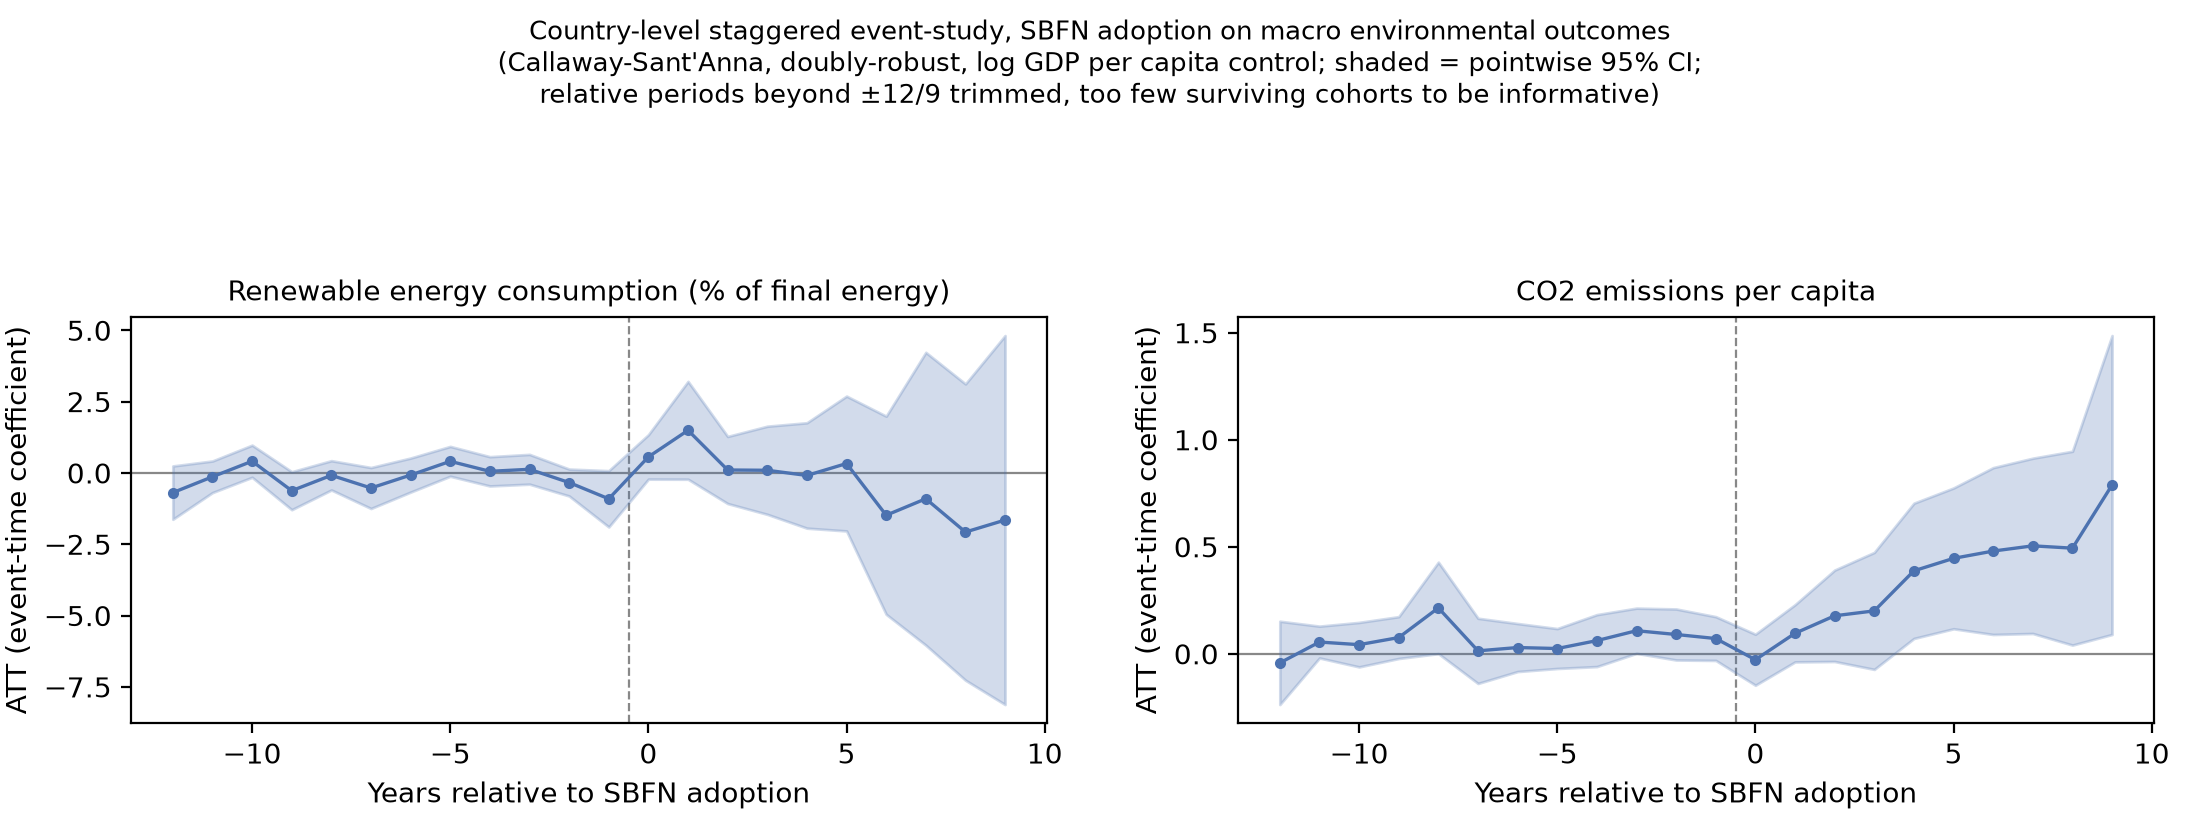
\includegraphics[width=0.95\textwidth]{../output/figures/fig6_macro_event_study.png}
\caption{Country-level staggered event-study, doubly-robust specification with log GDP per capita control. Shaded bands are pointwise 95\% confidence intervals; relative periods beyond $\pm$12/9 are trimmed for having too few surviving cohorts to be informative.}
\label{fig:macroevent}
\end{figure}

Two results, read together, do not support treating SBFN adoption as a country-level lever that visibly improves aggregate environmental outcomes -- which is itself informative, since this is the identification strategy best suited to answer that specific question directly. First, renewable energy share shows no effect distinguishable from zero in either specification, and the doubly-robust event-study profile (Figure~\ref{fig:macroevent}, left panel) is flat and precisely estimated on both sides of the adoption date: a clean null, not an underpowered one.

Second, CO2 emissions per capita shows a positive (i.e., the ``wrong-signed'' direction if SBFN adoption reduced emissions) and statistically significant association with adoption in every specification, but three features of the result argue against reading it causally. It shrinks by roughly 45\% (0.631 to 0.349) once we condition on log GDP per capita, indicating that a substantial share of the raw association is attributable to exactly the development-stage confound we set out to net out. The doubly-robust event-study profile (Figure~\ref{fig:macroevent}, right panel) shows a small, mostly flat pre-period with only two marginally significant leads, followed by a post-period effect that grows smoothly and monotonically from near zero at adoption to its largest magnitude nine to twelve years out -- a continuing-divergence pattern more consistent with SBFN-adopting economies already sitting on a different, faster-rising emissions trajectory than non-adopters (which a single covariate cannot fully absorb) than with a discrete policy-caused jump at the adoption date. And the naive TWFE estimate (0.901) is itself more than double the doubly-robust Callaway-Sant'Anna estimate (0.349), the same direction of bias documented in the staggered-DID literature \citep{goodmanbacon2021} and a useful internal illustration of why we lead with the more robust estimator throughout this section.

Both doubly-robust results are stable to the choice of comparison group: substituting not-yet-treated economies for never-treated economies leaves the CO2 estimate essentially unchanged (0.313 versus 0.349, both significant at conventional levels) and the renewable-energy null equally unchanged (0.653 versus 0.674, neither distinguishable from zero); Table~\ref{tab:macrodid} reports both. Neither conclusion in this section depends on which set of untreated economies serves as the counterfactual.

Neither result supports a ``green banking policy backfires'' reading, and neither supports a ``green banking policy works'' one. The more measured reading is that a macro-level design -- built using exactly the identification strategy (staggered adoption timing, a proper Callaway-Sant'Anna estimator, never-treated controls) this literature's own methodological expectations call for -- also does not produce clean evidence that SBFN adoption changes a country's aggregate environmental trajectory for the better, and the one statistically significant result we do find is more parsimoniously explained by which economies self-select into SBFN membership than by what the policy itself does once adopted. This is, we think, a genuinely different and complementary piece of evidence to Sections~\ref{sec:baseline}--\ref{sec:global}'s firm-level results, not a restatement of them: different data source, different unit of analysis, different outcome constructs, and, for the first time in this paper, an identification strategy that exploits exogenous variation in adoption \emph{timing} rather than relying on cross-sectional comparison across adopters and non-adopters. That it converges on the same substantive conclusion -- no clean evidence of a beneficial institutional effect -- from a design built specifically to meet a bar the paper's firm-level evidence cannot meet, strengthens rather than substitutes for the paper's central finding.

\section{Discussion}
\label{sec:discussion}

Put in plain economic terms, the paper's central finding is this: a firm holding a bank credit line is associated with an adoption probability roughly 13 percentage points higher than an otherwise-similar firm without one---an association net of observed controls, not a causally identified effect (Limitation 1)---and that gap is essentially unchanged whether the firm sits in an SBFN adopter or non-adopter, or across the full range of regulatory quality (Figure~\ref{fig:coefplot}). Firms in SBFN-adopting economies are, on average, 15--20 percentage points \emph{less} likely to have adopted a green practice at all---a level gap, not a slope gap.

This convergence is informative precisely because of how differently the evidence could have failed to agree. The primary and global samples share almost no economies, span different half-decades, use different outcome items, and reach institutional settings---high-income, non-SBFN economies such as Australia and Germany---the primary sample cannot touch. Section~\ref{sec:macrodid}'s country-level staggered event-study adds a third, independent test on top of this: a different data source, a different unit of analysis, and the paper's only design that exploits exogenous variation in adoption \emph{timing}. That it too finds no clean evidence of a beneficial institutional effect---a precise null on renewable-energy share, and a CO2 association that shrinks substantially once development stage is controlled for---is the hardest-to-dismiss evidence that this is a real feature of the data, not an artifact of any one sample, level of analysis, or estimator. (This is a distinct claim from H2/H3's firm-level moderation null---a main effect at country level, not a slope change at firm level---but evidence of the same kind.)

This complicates rather than confirms the implicit premise of a green-credit-policy literature disproportionately built on China's unusually mature, well-resourced guidelines \citep{li2023,huang2023,dai2025}. Our sample spans every stage of SBFN's own progression framework, from Jordan and the Kyrgyz Republic's initial ``Commitment'' to Mongolia's ``Advancing,'' and across that range we find no evidence that formal adoption changes how credit access translates into green investment. The causal forest's feature-importance decomposition (Section~\ref{sec:causalforest}) offers one redirection rather than a tidy answer: the heterogeneity that does exist is overwhelmingly a firm-size phenomenon (75.6\% of explained variance) rather than institutional (regulatory quality 19.9\%, SBFN 2.6\%)---though it does not resolve into a clean size gradient, so we can say where the heterogeneity sits without yet saying in which direction it runs. If the binding constraint is which firms can absorb a green investment's fixed costs once financed, rather than whether a supervisory guideline nudges banks to lend more broadly, a country-level mandate on the extensive margin of lending may be aimed at the wrong margin regardless of its own credibility.

``No interaction detected'' is not the same claim as ``no institutional complementarity exists,'' and we do not want the former to be read as settling the latter. Two alternative readings stay live: a linear interaction may be the wrong functional form for a genuinely threshold-shaped complementarity, given SBFN's own graded progression framework and our binary coding of it (Limitation 2); and the Worldwide Governance Indicators may simply not proxy the banking-supervisory capacity a green-lending guideline depends on (Limitation 5). We think our preferred reading---no complementarity through this channel---is best supported by the evidence, but hold it as the best current account rather than a claim that rules the alternatives out.

Two further limits are worth naming directly. First, SBFN guidelines could in principle be working on the \emph{extensive} margin of who obtains credit at all, rather than the \emph{intensive} margin our interaction terms test; testing that would require modeling credit access itself as a function of SBFN status, which our demand-side design does not do. Second, every outcome in this paper is firm-reported, and we cannot rule out a compliance-reporting-versus-practice gap between what firms report and what banks report to their own supervisor---a limit no firm-level survey instrument can fully resolve on its own. Read together with Section~\ref{sec:macrodid}, whose null is, to our knowledge, the first test of the SBFN framework's own theory of change against outcomes on the ground rather than its own tracked policy-stage progression, both point the same way: a framework can look like it is working by every measure the network itself tracks while the channel it is meant to move remains, on this evidence, unmoved.

The one interaction that clears a conventional significance threshold---a negative credit $\times$ SBFN effect for overdraft rather than term-credit access (Section~\ref{sec:results})---is more consistent with this redirection than with a simple policy failure: overdrafts finance working capital, not the long-horizon expenditure our outcome measures, so a supervisor successfully steering credit toward term instruments would produce exactly this pattern. We flag it as suggestive only: it is one significant coefficient among many tested, and does not survive a Benjamini--Hochberg correction at any conventional false discovery rate (Supplementary Table~S3).

Read against the broader themes of state capacity and policy credibility, our results sit closer to a state-capacity-is-necessary-but-firm-level-frictions-bind-independently story than a straightforward complementarity one. Regulatory quality raises the baseline propensity to adopt green practices, but is not the missing ingredient that lets a green banking guideline reshape the credit-to-green channel specifically. The binding constraint looks less like whether the supervising jurisdiction can make its guideline credible, and more like whether firms below a certain scale can absorb a green investment's fixed costs once credit is available---a question one level down from the one the SBFN framework is designed to answer.

\section{Conclusion}
\label{sec:conclusion}

This paper set out to test whether the wave of green banking policy adoption coordinated through the Sustainable Banking and Finance Network changes the relationship between firm-level access to finance and green investment behavior, and whether that depends on the regulatory capacity available to make the policy credible. Using harmonized WBES data across 41 economies (2018--2020), a four-country waste-minimization check, and an independently assembled 162-economy global sample (2021--2026) reaching for the first time into high-income, non-SBFN economies, we apply four escalating estimators and find five consistent results. First, bank credit access is robustly associated with green practice adoption, surviving every specification, subsample, and alternative-outcome check, and replicating in both the small waste-minimization sample and the full global sample. Second, neither SBFN adoption nor regulatory quality moderates that relationship under any estimator, on either sample, though both shift the general level of adoption directly in the primary sample. Third, where effect heterogeneity does exist, it sits at the level of firm size rather than country institutions. Fourth, this pattern replicates on a sample sharing almost no economies with the primary one, under a materially sharper identification strategy. Fifth, and most importantly for the paper's credibility, an independent country-level staggered event-study (Section~\ref{sec:macrodid})---a main-effect test, not a repeat of the firm-level moderation null---likewise finds no clean evidence that SBFN adoption improves aggregate environmental outcomes, the single strongest evidence that this null is a real feature of the data rather than an artifact of any one sample, data source, level of analysis, or estimator.

For policy, the implication is not that green banking guidelines are ineffective, but that our evidence does not support treating them as a lever for widening the green-investment gap between financed and unfinanced firms---the margin most of this literature implicitly assumes they operate on. If our tentative loan-tenor reading of the overdraft result is correct, policymakers may find more traction focusing on the term-lending instruments that actually finance green capital expenditure, and on complementary measures---technical assistance, matching grants, credit guarantees---that address smaller firms' absorptive-capacity constraints directly.

We close with seven limitations. First, both firm-level samples are single cross-sections (Section~\ref{sec:methodology} explains why a genuine panel does not exist for this outcome): they cannot rule out reverse causality or unobserved country characteristics correlated with both SBFN adoption and baseline green-adoption propensity, and the global sample's fixed effects sharpen this only for the interaction terms, not the credit main effect. Second, SBFN membership is a binary proxy for what the network's own framework treats as a graded process; the global sample's regional roster entries (the CEMAC and Eastern Caribbean groupings, Section~\ref{sec:methodology}) additionally rest on an inference about coverage rather than an explicit per-country statement. Third, the four-economy waste-minimization check cannot re-test the SBFN contrast (three of its four economies are members) and combines non-identical outcome items by construction of WBES's own shortened module design---a data-availability constraint, not a methodological choice. Fourth, the global sample's CO2-monitoring outcome is a single item, narrower than the primary sample's seven-item composite; that the same pattern holds on it is reassuring but does not establish it would hold on a richer measure. Fifth, the Worldwide Governance Indicators measure is a broad governance indicator, not a banking-supervision-specific capacity measure. Sixth, our design tests only the intensive margin of the credit-to-green channel and cannot rule out that SBFN policy operates on the extensive margin of who obtains credit in the first place---a margin our realized-access measure cannot observe, since some firms decline formal credit altogether \citep{jin2026}---nor distinguish firm-reported practice adoption from a bank-compliance-reporting gap (Section~\ref{sec:discussion}). Seventh, Section~\ref{sec:macrodid}'s event-study is an ecological-level test of a related but distinct question; its one significant result (CO2 per capita) is netted against a single covariate, and we cannot rule out that a richer set of development-stage controls would shrink it further, or that some genuine, small, confounded relationship remains. We leave each of these to future work.

\section*{Declaration of generative AI and AI-assisted technologies in the manuscript preparation process}

During the preparation of this work the author(s) used AI-assisted tools to help polish the writing. After using these tools, the author(s) reviewed and edited the content as needed and take full responsibility for the content of the published article.

\section*{Supplementary material}

The full per-economy SBFN membership and regulatory-quality coding for both samples, Bayesian
convergence diagnostics, the global sample's SBFN membership by region, and the additional
robustness checks and multiple-testing correction referenced above (Section~\ref{sec:extension},
\ref{sec:robustness}) are reported in the Supplementary Material accompanying this submission.

\subsection*{Data availability}

Data in support of the findings of this study is available from the corresponding author upon reasonable request, subject to the World Bank Enterprise Surveys' own terms of use for the underlying firm-level microdata (enterprisesurveys.org, free registration required), including the standardized cross-country database and Productivity Database underlying the global sample. The country-level SBFN policy-status (including the SBFN data portal's member roster underlying the global sample) and Worldwide Governance Indicators datasets constructed for this paper, the country-year World Development Indicators panel and Callaway-Sant'Anna event-study code underlying Section~\ref{sec:macrodid} (all freely redistributable, no registration required), together with the full analysis and replication code, are available at \url{https://github.com/vinhqdang/green-credit-substitution}.

% Reference list in author-date format.
% Generated from references.bib; kept inline so the submitted source is self-contained.
\begin{thebibliography}{99}

\bibitem[Acemoglu et al.(2001)]{acemoglu2001}
Acemoglu, D., Johnson, S., \& Robinson, J. A. (2001). The colonial origins of comparative development: An empirical investigation. \emph{American Economic Review}, \emph{91}(5), 1369--1401. \url{https://doi.org/10.1257/aer.91.5.1369}

\bibitem[Aristei and Gallo(2023)]{aristei2023}
Aristei, D., \& Gallo, M. (2023). Green management, access to credit, and firms' vulnerability to the COVID-19 crisis. \emph{Small Business Economics}, 1--33. \url{https://doi.org/10.1007/s11187-023-00759-1}

\bibitem[Asif et al.(2025)]{asif2025}
Asif, M., Dhamija, A., Khan, W., Johri, A., \& Wasiq, M. (2025). Factors affecting adoption of green practices by food firms: Evidences from the World Bank Enterprises Survey. \emph{Clean Technologies and Environmental Policy}, \emph{27}(9), 4841--4858. \url{https://doi.org/10.1007/s10098-024-03122-4}

\bibitem[Athey and Imbens(2019)]{athey2019}
Athey, S., \& Imbens, G. W. (2019). Machine learning methods that economists should know about. \emph{Annual Review of Economics}, \emph{11}(1), 685--725. \url{https://doi.org/10.1146/annurev-economics-080217-053433}

\bibitem[Athey et al.(2019)]{athey2019grf}
Athey, S., Tibshirani, J., \& Wager, S. (2019). Generalized random forests. \emph{The Annals of Statistics}, \emph{47}(2), 1148--1178. \url{https://doi.org/10.1214/18-AOS1709}

\bibitem[Bambe et al.(2026)]{bambe2026}
Bambe, B. W. W., Combes, J.-L., Kouassi, B.-V., \& Schwartz, S. (2026). Environmental policy stringency and firm efficiency in developing countries. \emph{Small Business Economics}, \emph{66}(3), 1163--1182. \url{https://doi.org/10.1007/s11187-025-01128-w}

\bibitem[Beck et al.(2005)]{beck2005}
Beck, T., Demirg{\"u}{\c{c}}-Kunt, A., \& Maksimovic, V. (2005). Financial and legal constraints to growth: Does firm size matter? \emph{The Journal of Finance}, \emph{60}(1), 137--177. \url{https://doi.org/10.1111/j.1540-6261.2005.00727.x}

\bibitem[Beck et al.(2008)]{beck2008}
Beck, T., Demirg{\"u}{\c{c}}-Kunt, A., \& Maksimovic, V. (2008). Financing patterns around the world: Are small firms different? \emph{Journal of Financial Economics}, \emph{89}(3), 467--487. \url{https://doi.org/10.1016/j.jfineco.2007.10.005}

\bibitem[Callaway and Sant'Anna(2021)]{callaway2021}
Callaway, B., \& Sant'Anna, P. H. C. (2021). Difference-in-differences with multiple time periods. \emph{Journal of Econometrics}, \emph{225}(2), 200--230. \url{https://doi.org/10.1016/j.jeconom.2020.12.001}

\bibitem[Cameron and Miller(2015)]{cameron2015}
Cameron, A. C., \& Miller, D. L. (2015). A practitioner's guide to cluster-robust inference. \emph{Journal of Human Resources}, \emph{50}(2), 317--372. \url{https://doi.org/10.3368/jhr.50.2.317}

\bibitem[Chernozhukov et al.(2018)]{chernozhukov2018}
Chernozhukov, V., Chetverikov, D., Demirer, M., Duflo, E., Hansen, C., Newey, W., \& Robins, J. (2018). Double/debiased machine learning for treatment and structural parameters. \emph{The Econometrics Journal}, \emph{21}(1), C1--C68. \url{https://doi.org/10.1111/ectj.12097}

\bibitem[Chi and Yang(2023)]{chi2023}
Chi, Y., \& Yang, Y. (2023). Green finance and green transition by enterprises: An exploration of market-oriented governance mechanisms. \emph{Borsa Istanbul Review}, \emph{23}(3), 628--646. \url{https://doi.org/10.1016/j.bir.2023.01.003}

\bibitem[Costa et al.(2024)]{costa2024}
Costa, H., Demmou, L., Franco, G., \& Lamp, S. (2024). The role of financing constraints and environmental policy on green investment. \emph{Economics Letters}, \emph{239}, Article 111741. \url{https://doi.org/10.1016/j.econlet.2024.111741}

\bibitem[Dai et al.(2025)]{dai2025}
Dai, Q., He, J., Guo, Z., Zheng, Y., \& Zhang, Y. (2025). Green finance for sustainable development: Analyzing the effects of green credit on high-polluting firms' environmental performance. \emph{Humanities and Social Sciences Communications}, \emph{12}(1), Article 854. \url{https://doi.org/10.1057/s41599-025-05218-8}

\bibitem[De Haas et al.(2025)]{dehaas2025}
De Haas, R., Martin, R., Mu{\^u}ls, M., \& Schweiger, H. (2025). Managerial and financial barriers to the green transition. \emph{Management Science}, \emph{71}(4), 2890--2921. \url{https://doi.org/10.1287/mnsc.2023.00772}

\bibitem[Demirg{\"u}{\c{c}}-Kunt and Maksimovic(1998)]{demirguckunt1998}
Demirg{\"u}{\c{c}}-Kunt, A., \& Maksimovic, V. (1998). Law, finance, and firm growth. \emph{The Journal of Finance}, \emph{53}(6), 2107--2137. \url{https://doi.org/10.1111/0022-1082.00084}

\bibitem[Gao et al.(2022)]{gao2022}
Gao, D., Mo, X., Duan, K., \& Li, Y. (2022). Can green credit policy promote firms' green innovation? Evidence from China. \emph{Sustainability}, \emph{14}(7), Article 3911. \url{https://doi.org/10.3390/su14073911}

\bibitem[Gelman and Hill(2007)]{gelman2007}
Gelman, A., \& Hill, J. (2007). \emph{Data analysis using regression and multilevel/hierarchical models}. Cambridge University Press. \url{https://doi.org/10.1017/CBO9780511790942}

\bibitem[Gelman et al.(2020)]{gelman2020}
Gelman, A., Hill, J., \& Vehtari, A. (2020). \emph{Regression and other stories}. Cambridge University Press. \url{https://doi.org/10.1017/9781139161879}

\bibitem[Ghosh and Dutta(2022)]{ghosh2022}
Ghosh, D., \& Dutta, M. (2022). Environmental behaviour under credit constraints -- evidence from panel of Indian manufacturing firms. \emph{Structural Change and Economic Dynamics}, \emph{63}, 490--500. \url{https://doi.org/10.1016/j.strueco.2022.07.004}

\bibitem[Goodman-Bacon(2021)]{goodmanbacon2021}
Goodman-Bacon, A. (2021). Difference-in-differences with variation in treatment timing. \emph{Journal of Econometrics}, \emph{225}(2), 254--277. \url{https://doi.org/10.1016/j.jeconom.2021.03.014}

\bibitem[Hall and Soskice(2001)]{hallsoskice2001}
Hall, P. A., \& Soskice, D. (2001). \emph{Varieties of capitalism: The institutional foundations of comparative advantage}. Oxford University Press.

\bibitem[Huang et al.(2023)]{huang2023}
Huang, Z., Gao, N., \& Jia, M. (2023). Green credit and its obstacles: Evidence from China's green credit guidelines. \emph{Journal of Corporate Finance}, \emph{82}, Article 102441. \url{https://doi.org/10.1016/j.jcorpfin.2023.102441}

\bibitem[International Finance Corporation / Sustainable Banking and Finance Network(2025)]{ifc2025sbfn}
International Finance Corporation / Sustainable Banking and Finance Network (2025). \emph{Sustainable Banking and Finance Network global progress report 2025}. World Bank Group / IFC. \url{https://documents1.worldbank.org/curated/en/099634202132617625/pdf/IDU-3c06eadd-dd50-446d-a6d0-3fe3907bf5d5.pdf}

\bibitem[Jia et al.(2026)]{jia2026}
Jia, S., Farooq, U., Alomair, A., \& Aljughaiman, A. A. (2026). Credit with a climate purpose: Does green credit policy accelerate sustainable production in BRICS? \emph{Borsa Istanbul Review}, \emph{26}(3), Article 100817. \url{https://doi.org/10.1016/j.bir.2026.100817}

\bibitem[Jin(2026)]{jin2026}
Jin, W. (2026). Choosing not to borrow: Imprinting effects of informality on firms' credit self-rationing. \emph{Borsa Istanbul Review}, \emph{26}(2), Article 100785. \url{https://doi.org/10.1016/j.bir.2026.100785}

\bibitem[Kalantzis et al.(2022)]{kalantzis2022}
Kalantzis, F., Schweiger, H., \& Dominguez, S. (2022). \emph{Green investment by firms: Finance or climate driven?} EBRD Working Paper No. 268. \url{https://doi.org/10.2139/ssrn.4132545}

\bibitem[Khairunnessa et al.(2021)]{khairunnessa2021}
Khairunnessa, F., Vazquez-Brust, D. A., \& Yakovleva, N. (2021). A review of the recent developments of green banking in Bangladesh. \emph{Sustainability}, \emph{13}(4), Article 1904. \url{https://doi.org/10.3390/su13041904}

\bibitem[La Porta et al.(1998)]{laporta1998}
La Porta, R., Lopez-de-Silanes, F., Shleifer, A., \& Vishny, R. (1998). Law and finance. \emph{Journal of Political Economy}, \emph{106}(6), 1113--1155. \url{https://doi.org/10.1086/250042}

\bibitem[Levine(2005)]{levine2005}
Levine, R. (2005). Finance and growth: Theory and evidence. In P. Aghion, \& S. Durlauf (Eds.), \emph{Handbook of economic growth} (Vol. 1A, pp. 865--934). Elsevier. \url{https://doi.org/10.1016/S1574-0684(05)01012-9}

\bibitem[Li et al.(2023)]{li2023}
Li, C., Feng, X., Li, X., \& Zhou, Y. (2023). Effect of green credit policy on energy firms' growth: Evidence from China. \emph{Economic Research-Ekonomska Istra{\v{z}}ivanja}, \emph{36}(2). \url{https://doi.org/10.1080/1331677X.2023.2177701}

\bibitem[Li et al.(2024)]{li2024}
Li, C., Liu, Z., Song, R., \& Zhang, Y.-J. (2024). The impact of green credit guidelines on environmental performance: Firm-level evidence from China. \emph{Technological Forecasting and Social Change}, \emph{205}, Article 123524. \url{https://doi.org/10.1016/j.techfore.2024.123524}

\bibitem[Nguyen and Phan(2025)]{nguyen2025}
Nguyen, M. P., \& Phan, A. (2025). Impact of green credit policy on the operation of Vietnamese commercial banks: An empirical study using difference-in-differences model. \emph{PLOS One}, \emph{20}(10), Article e0333759. \url{https://doi.org/10.1371/journal.pone.0333759}

\bibitem[Phan(2026)]{phan2026}
Phan, Q. T. (2026). The impact of green economy practices on firm innovation using data from the World Bank Enterprise Surveys. \emph{Discover Sustainability}, \emph{7}(1), Article 848. \url{https://doi.org/10.1007/s43621-026-03226-5}

\bibitem[Salvatier et al.(2016)]{salvatier2016}
Salvatier, J., Wiecki, T. V., \& Fonnesbeck, C. (2016). Probabilistic programming in Python using PyMC3. \emph{PeerJ Computer Science}, \emph{2}, Article e55. \url{https://doi.org/10.7717/peerj-cs.55}

\bibitem[Shi et al.(2024)]{shi2024}
Shi, Y., Zhu, Q., \& Khan, M. A. (2024). The efficacy of green finance for environmental sustainability: Does control of corruption makes a difference? \emph{Borsa Istanbul Review}, \emph{24}(6), 1179--1189. \url{https://doi.org/10.1016/j.bir.2024.07.002}

\bibitem[Siewers et al.(2024)]{siewers2024}
Siewers, S., Mart{\'i}nez-Zarzoso, I., \& Baghdadi, L. (2024). Global value chains and firms' environmental performance. \emph{World Development}, \emph{173}, Article 106395. \url{https://doi.org/10.1016/j.worlddev.2023.106395}

\bibitem[Tran et al.(2026)]{tran2026}
Tran, T. T. C., Nguyen, L., \& Do, T. K. (2026). The impact of fintech credit on green innovation: International evidence. \emph{Journal of Economics and Development}, \emph{28}(2), 111--127. \url{https://doi.org/10.1108/JED-05-2025-0177}

\bibitem[Truong(2026)]{truong2026}
Truong, D. D. (2026). Does access to finance condition firms' green investment responses to environmental pressure? Evidence from Vietnam. \emph{PLOS One}, \emph{21}(5), Article e0341960. \url{https://doi.org/10.1371/journal.pone.0341960}

\bibitem[B. Ullah(2025)]{ullah2025}
Ullah, B. (2025). Corporate environmental responsibility and financial constraints for unlisted SMEs. \emph{Global Finance Journal}, \emph{67}, Article 101176. \url{https://doi.org/10.1016/j.gfj.2025.101176}

\bibitem[W. Ullah et al.(2024)]{ullahw2024}
Ullah, W., Zubir, A. S. M., \& Ariff, A. M. (2024). Exploring the moderating effect of regulatory quality on the relationship between financial development and economic growth/economic volatility for developed and developing countries. \emph{Borsa Istanbul Review}, \emph{24}(5), 934--944. \url{https://doi.org/10.1016/j.bir.2024.04.015}

\bibitem[Wager and Athey(2018)]{wager2018}
Wager, S., \& Athey, S. (2018). Estimation and inference of heterogeneous treatment effects using random forests. \emph{Journal of the American Statistical Association}, \emph{113}(523), 1228--1242. \url{https://doi.org/10.1080/01621459.2017.1319839}

\end{thebibliography}

\end{document}
